\documentclass[11pt]{article}
\usepackage[margin=1in]{geometry}
\usepackage[T1]{fontenc}
\usepackage{lmodern}
\usepackage{microtype}
\usepackage{amsmath,amssymb,amsthm,mathtools}
\usepackage{booktabs,graphicx,xcolor,enumitem,listings}
\usepackage[colorlinks=true,linkcolor=blue!50!black,citecolor=blue!50!black,urlcolor=blue!50!black]{hyperref}

\graphicspath{{figures/}}
\newcommand{\SMeanOffspring}{0.70}
\newcommand{\STheoryMeanN}{3.333}
\newcommand{\SEmpMeanN}{3.314}
\newcommand{\SEmpMeanNTrunc}{2.765}
\newcommand{\SEmpMaxN}{99}
\newcommand{\SNSamples}{50{,}000}
\newcommand{\SAcceptRate}{0.686}
\newcommand{\SRejectUnnatural}{0.312}
\newcommand{\SRejectSize}{0.002}
\newcommand{\SQMeanOffspring}{0.82}
\newcommand{\SChainMeanP}{0.975}
\newcommand{\SChainMeanQ}{1.612}
\newcommand{\SChainMeanIS}{1.594}
\newcommand{\STailP}{0.018}
\newcommand{\STailQ}{0.065}
\newcommand{\SESS}{14{,}540}
\newcommand{\SISM}{20{,}000}
\newcommand{\SUniqueOf}{400}

\newcommand{\TExProblem}{x^{2} \sin\left(e^{3 x}\right)}
\newcommand{\TExDerivative}{2 x \sin\left(e^{3 x}\right) + 3 x^{2} \cos\left(e^{3 x}\right) e^{3 x}}
\newcommand{\TNProblems}{3{,}000}
\newcommand{\TNVerified}{2{,}989}
\newcommand{\TNInconclusive}{11}
\newcommand{\TRhoNSteps}{0.91}
\newcommand{\TRhoInOut}{0.89}
\newcommand{\TMeanSteps}{8.6}
\newcommand{\TMaxSwell}{5.4}
\newcommand{\TMedSwell}{1.60}
\newcommand{\TSwellSlope}{1.51}
\newcommand{\TFracChain}{0.71}
\newcommand{\TFracProduct}{0.17}
\newcommand{\TFracQuotient}{0.12}
\newcommand{\TFracChainTwo}{0.31}

\newcommand{\FNFeatures}{17}
\newcommand{\FNProblems}{3{,}000}
\newcommand{\FCond}{557}
\newcommand{\FEigMax}{6.78}
\newcommand{\FEigMin}{0.012}
\newcommand{\FNinetyPct}{10}
\newcommand{\FTopPairA}{n\_chain}
\newcommand{\FTopPairB}{max\_chain\_depth}
\newcommand{\FTopCorr}{0.92}
\newcommand{\FCorrSizePower}{0.78}
\newcommand{\FCorrChainProd}{0.39}
\newcommand{\FNDistinct}{2{,}095}
\newcommand{\FBiggestClass}{37}
\newcommand{\FTwinA}{4 x^{4}}
\newcommand{\FTwinB}{3 x^{4}}
\newcommand{\FCollideA}{\cos\left(x^{2}\right)}
\newcommand{\FCollideB}{\sin\left(x^{2}\right)}
\newcommand{\FFracCIPZero}{0.76}

\newcommand{\BNItems}{200}
\newcommand{\BDeltaSD}{1.45}
\newcommand{\BDeltaMin}{-2.7}
\newcommand{\BDeltaMax}{5.0}
\newcommand{\BMLEExists}{exists}
\newcommand{\BNPerfect}{0}
\newcommand{\BLTwo}{0.1}
\newcommand{\BPriorSD}{3.2}
\newcommand{\BM}{4{,}000}
\newcommand{\BPerItem}{40}
\newcommand{\BNewtonIters}{6}
\newcommand{\BRMSE}{0.48}
\newcommand{\BMeanSE}{0.44}
\newcommand{\BMeanSENaive}{0.50}
\newcommand{\BCoverage}{94}
\newcommand{\BSpearman}{0.929}
\newcommand{\BSumTheta}{1e-14}
\newcommand{\BGDIters}{300}
\newcommand{\BGDToTen}{220}
\newcommand{\BHessCond}{113}
\newcommand{\BRateSlope}{-0.51}
\newcommand{\BExistsTwo}{0.0}
\newcommand{\BExistsEight}{0.0}
\newcommand{\BExistsThirtyTwo}{0.0}
\newcommand{\BSmallKRMSE}{1.39}
\newcommand{\BLargeKRMSE}{0.25}
\newcommand{\BLargeKTheory}{0.24}

\newcommand{\EFeatAcc}{0.747}
\newcommand{\EBootLo}{0.716}
\newcommand{\EBootHi}{0.781}
\newcommand{\EBootHalf}{0.033}
\newcommand{\ENaiveHalf}{0.013}
\newcommand{\EWidthRatio}{2.4}
\newcommand{\ENTest}{200}
\newcommand{\ENTestPairs}{4{,}000}
\newcommand{\ESpearman}{0.890}
\newcommand{\EKendall}{0.720}
\newcommand{\EDeltaSD}{1.50}
\newcommand{\ECeilHere}{0.787}

\newcommand{\GCeiling}{0.776}
\newcommand{\GFeatCeiling}{0.754}
\newcommand{\GAccSmall}{0.719}
\newcommand{\GAccTwoHundred}{0.747}
\newcommand{\GAccLarge}{0.753}
\newcommand{\GSizeOnlyLarge}{0.711}
\newcommand{\GDerivOnlyLarge}{0.742}
\newcommand{\GLamSmall}{20.8}
\newcommand{\GLamLarge}{100}
\newcommand{\GLamRatioSmall}{0.83}
\newcommand{\GLamRatioLarge}{0.031}
\newcommand{\GNTrainProblems}{350}
\newcommand{\GNTestProblems}{150}
\newcommand{\GWithinOne}{200}
\newcommand{\GPerProblemAtTwoHundred}{1.1}
\newcommand{\GCovered}{13}
\newcommand{\GCoveredBoot}{14}
\newcommand{\GSERatio}{1.4}
\newcommand{\GMissed}{\code{n\_chain}, \code{n\_trig}, \code{n\_exp}, \code{n\_ln}}
\newcommand{\GNFeat}{17}
\newcommand{\GRepCovLaplace}{90}
\newcommand{\GRepCovBoot}{99}
\newcommand{\GRepSERatio}{1.9}
\newcommand{\GQuotW}{0.48}
\newcommand{\GQuotSE}{0.19}
\newcommand{\GQuotPlanted}{0.55}
\newcommand{\GSizeW}{0.018}
\newcommand{\GSizeSE}{0.010}
\newcommand{\GCVBestSmall}{31.6228}

\newcommand{\HProbitScale}{1.702}
\newcommand{\HProbitGap}{0.0095}
\newcommand{\HCeilAtSeventy}{0.780}
\newcommand{\HSAtSeventy}{1.43}
\newcommand{\HCeilAtEighty}{0.858}
\newcommand{\HSAtEighty}{2.52}
\newcommand{\HCeilAtNinety}{0.930}
\newcommand{\HSAtNinety}{5.47}

\newcommand{\RNJudg}{330}
\newcommand{\RNRepeats}{30}
\newcommand{\RNTies}{56}
\newcommand{\RTiePct}{17}
\newcommand{\RNProblemsSeen}{249}
\newcommand{\RNPool}{300}
\newcommand{\RLeftRate}{0.504}
\newcommand{\RMedianRT}{1.9}
\newcommand{\RNFlags}{0}
\newcommand{\RNAutoFlags}{12}
\newcommand{\RAgreeAll}{25/30}
\newcommand{\RAgreeDD}{20/22}
\newcommand{\RDisagreeTie}{3}
\newcommand{\RDisagreeTotal}{5}
\newcommand{\RAgreeDDRate}{0.91}
\newcommand{\RAgreeDDLo}{0.74}
\newcommand{\RAgreeDDHi}{0.98}
\newcommand{\RCeilDD}{0.94}
\newcommand{\RCeilDDLo}{0.81}
\newcommand{\RCeilDDHi}{0.99}
\newcommand{\RAccFull}{0.914}
\newcommand{\RLLFull}{0.310}
\newcommand{\RAccFullLo}{0.843}
\newcommand{\RAccFullHi}{0.961}
\newcommand{\RLLFullLo}{0.229}
\newcommand{\RLLFullHi}{0.396}
\newcommand{\RAccDeriv}{0.925}
\newcommand{\RLLDeriv}{0.378}
\newcommand{\RAccDerivLo}{0.868}
\newcommand{\RAccDerivHi}{0.972}
\newcommand{\RLLDerivLo}{0.274}
\newcommand{\RLLDerivHi}{0.514}
\newcommand{\RLLDiffLo}{-0.183}
\newcommand{\RLLDiffHi}{0.000}
\newcommand{\RDFAtTwoHundred}{10.8}
\newcommand{\RGapPredTwoHundred}{0.054}
\newcommand{\RGapObsTwoHundred}{0.053}
\newcommand{\RGapPredTwentyFive}{0.229}
\newcommand{\RGapObsTwentyFive}{0.148}
\newcommand{\RAccFullTwentyFive}{0.903}
\newcommand{\RAccDerivTwentyFive}{0.925}
\newcommand{\RLLFullTwentyFive}{0.381}
\newcommand{\RLLDerivTwentyFive}{0.484}
\newcommand{\RLamAll}{3.16228}
\newcommand{\RQuotW}{2.9}
\newcommand{\RQuotLapLo}{1.4}
\newcommand{\RQuotLapHi}{4.5}
\newcommand{\RQuotLo}{1.2}
\newcommand{\RQuotHi}{4.5}
\newcommand{\RQuotFracPos}{100.0}
\newcommand{\RRealSERatio}{1.0}
\newcommand{\RNSig}{4}
\newcommand{\RQuotSmallLam}{4.6}
\newcommand{\RQuotLargeLam}{1.3}
\newcommand{\RTopStd}{\code{n\_quotient}, \code{n\_chain}, \code{n\_power}, \code{depth}}
\newcommand{\RRhoScoreDeriv}{0.97}
\newcommand{\RNDropped}{26}
\newcommand{\RAccKeep}{0.923}
\newcommand{\RLLKeep}{0.299}
\newcommand{\RQuotKeep}{2.9}
\newcommand{\RQuotKeepLo}{1.2}
\newcommand{\RQuotKeepHi}{4.6}
\newcommand{\RFracQuot}{13}
\newcommand{\RTieLowGap}{54}
\newcommand{\RTieHighGap}{0}
\newcommand{\RRTLowGap}{2.4}
\newcommand{\RRTHighGap}{1.3}
\newcommand{\RNWrong}{25}

\newcommand{\QLinTruthLinSmall}{0.552}
\newcommand{\QLinTruthBoostSmall}{0.580}
\newcommand{\QLinTruthLinLarge}{0.537}
\newcommand{\QLinTruthBoostLarge}{0.541}
\newcommand{\QIntTruthLinLarge}{0.520}
\newcommand{\QIntTruthBoostLarge}{0.515}
\newcommand{\QIntTruthOracle}{0.511}
\newcommand{\QLinTruthOracle}{0.495}
\newcommand{\QIntCross}{400}
\newcommand{\QNJudg}{330}
\newcommand{\QRealAccLin}{0.909}
\newcommand{\QRealLLLin}{0.304}
\newcommand{\QRealAccBoost}{0.938}
\newcommand{\QRealLLBoost}{0.290}
\newcommand{\QRealDiffLo}{-0.065}
\newcommand{\QRealDiffHi}{0.024}
\newcommand{\QRealNTrees}{65}
\newcommand{\QBestTreesDepthOne}{54}
\newcommand{\QBestLLDepthOne}{0.303}
\newcommand{\QBestTreesDepthTwo}{50}
\newcommand{\QBestLLDepthTwo}{0.312}
\newcommand{\QBestTreesDepthFour}{68}
\newcommand{\QBestLLDepthFour}{0.316}
\newcommand{\QFinalLLDepthFour}{0.355}
\newcommand{\QFinalTrainDepthFour}{0.150}
\newcommand{\QGainTop}{\code{deriv\_size} (43\%), \code{size} (20\%), \code{depth} (12\%)}

\newcommand{\AVarNeedsForHundred}{103}
\newcommand{\ASavingHundred}{-3}
\newcommand{\AVarNeedsForTwoHundred}{153}
\newcommand{\ASavingTwoHundred}{23}
\newcommand{\ALLRandHundred}{0.570}
\newcommand{\ALLRandFinal}{0.548}
\newcommand{\AAccRandHundred}{0.703}
\newcommand{\AGapRand}{1.69}
\newcommand{\AMaxUseRand}{7}
\newcommand{\ALLUncHundred}{0.634}
\newcommand{\ALLUncFinal}{0.650}
\newcommand{\AAccUncHundred}{0.690}
\newcommand{\AGapUnc}{0.77}
\newcommand{\AMaxUseUnc}{9}
\newcommand{\ALLInfoHundred}{0.578}
\newcommand{\ALLInfoFinal}{0.557}
\newcommand{\AAccInfoHundred}{0.713}
\newcommand{\AGapInfo}{0.96}
\newcommand{\AMaxUseInfo}{20}
\newcommand{\ALLVarHundred}{0.573}
\newcommand{\ALLVarFinal}{0.541}
\newcommand{\AAccVarHundred}{0.714}
\newcommand{\AGapVar}{1.38}
\newcommand{\AMaxUseVar}{13}
\newcommand{\ASeeds}{8}
\newcommand{\ALLRandSixty}{0.586}
\newcommand{\ALLRandTwoHundred}{0.555}
\newcommand{\ALLUncSixty}{0.632}
\newcommand{\ALLUncTwoHundred}{0.663}
\newcommand{\ALLInfoSixty}{0.571}
\newcommand{\ALLInfoTwoHundred}{0.567}
\newcommand{\ALLVarSixty}{0.577}
\newcommand{\ALLVarTwoHundred}{0.548}
\newcommand{\ADiffVarSixty}{-0.009}
\newcommand{\ADiffSEVarSixty}{0.010}
\newcommand{\AWinsVarSixty}{6}
\newcommand{\ADiffVarTwoHundred}{-0.007}
\newcommand{\ADiffSEVarTwoHundred}{0.004}
\newcommand{\AWinsVarTwoHundred}{6}
\newcommand{\ADiffVarThreeHundred}{-0.007}
\newcommand{\ADiffSEVarThreeHundred}{0.006}
\newcommand{\AWinsVarThreeHundred}{6}
\newcommand{\ADiffInfoSixty}{-0.014}
\newcommand{\ADiffSEInfoSixty}{0.009}
\newcommand{\AWinsInfoSixty}{6}
\newcommand{\ADiffInfoTwoHundred}{+0.012}
\newcommand{\ADiffSEInfoTwoHundred}{0.012}
\newcommand{\AWinsInfoTwoHundred}{3}
\newcommand{\ADiffInfoThreeHundred}{+0.009}
\newcommand{\ADiffSEInfoThreeHundred}{0.010}
\newcommand{\AWinsInfoThreeHundred}{5}
\newcommand{\ANTotal}{300}
\newcommand{\ABatch}{5}
\newcommand{\ANReal}{300}
\newcommand{\AReplayRandSixty}{0.342}
\newcommand{\AReplayRandEnd}{0.324}
\newcommand{\AReplayInfoSixty}{0.331}
\newcommand{\AReplayInfoEnd}{0.320}
\newcommand{\AReplayVarSixty}{0.332}
\newcommand{\AReplayVarEnd}{0.321}
\newcommand{\AReplayVarReach}{80}

\newcommand{\NPreTime}{15}
\newcommand{\NNPre}{5{,}000}
\newcommand{\NPreNodes}{13{,}713}
\newcommand{\NRsqDerivSize}{0.94}
\newcommand{\NRsqNChain}{0.96}
\newcommand{\NRsqMaxChainDepth}{0.88}
\newcommand{\NRsqNQuotient}{0.95}
\newcommand{\NRsqChainInProduct}{0.81}
\newcommand{\NRsqMin}{0.68}
\newcommand{\NRsqMinName}{n\_neg\_exp}
\newcommand{\NNParams}{3{,}104}
\newcommand{\NSynOracle}{0.465}
\newcommand{\NSynLinSmall}{0.533}
\newcommand{\NSynLinLarge}{0.509}
\newcommand{\NSynScratchSmall}{0.701}
\newcommand{\NSynScratchLarge}{0.641}
\newcommand{\NSynLPFTSmall}{0.519}
\newcommand{\NSynLPFTLarge}{0.512}
\newcommand{\NScratchCatchUp}{more than 10{,}000}
\newcommand{\NNJudg}{337}
\newcommand{\NLPFTvsLinLo}{-0.052}
\newcommand{\NLPFTvsLinHi}{0.025}
\newcommand{\NRealLLLin}{0.310}
\newcommand{\NRealLLLPFT}{0.297}
\newcommand{\NRealLLScratch}{0.622}
\newcommand{\NRealLLFrozen}{0.332}
\newcommand{\NRealLLNaive}{0.420}
\newcommand{\NRealAccScratch}{0.676}
\newcommand{\NScratchBestEpoch}{8}
\newcommand{\NScratchTrainEnd}{0.137}
\newcommand{\NScratchValEnd}{1.189}
\newcommand{\NScratchValBest}{0.681}
\newcommand{\NNTrPairsFold}{218}

\newcommand{\XNJudg}{346}
\newcommand{\XNGroups}{7}
\newcommand{\XNCoalitions}{128}
\newcommand{\XTopLin}{chain rule}
\newcommand{\XSecondLin}{size}
\newcommand{\XTopShareLin}{30}
\newcommand{\XTopBst}{size}
\newcommand{\XSecondBst}{chain rule}
\newcommand{\XTopShareBst}{61}
\newcommand{\XRhoLinBst}{0.93}
\newcommand{\XGainTopGroup}{size}
\newcommand{\XGainTopShare}{77}
\newcommand{\XQuotRankBst}{5}
\newcommand{\XQuotRankGain}{6}
\newcommand{\XEffErr}{2e-15}
\newcommand{\XSampSlope}{-0.48}
\newcommand{\XSampErrTwenty}{0.033}
\newcommand{\XWFHard}{x^{-1} + x^{1/2} + \frac{\sqrt{4 x^{3}}}{2 x^{3/2}} + 2}
\newcommand{\XWFEasy}{x^{4} + x^{2} + \tan\left(x^{4} - 4\right)}
\newcommand{\XWFGap}{2.67}
\newcommand{\XWFProb}{0.94}


\theoremstyle{definition}
\newtheorem{definition}{Definition}[section]
\newtheorem{exercise}{Exercise}[section]
\theoremstyle{plain}
\newtheorem{theorem}[definition]{Theorem}
\newtheorem{proposition}[definition]{Proposition}
\theoremstyle{remark}
\newtheorem{remark}[definition]{Remark}

\newcommand{\R}{\mathbb{R}}
\newcommand{\E}{\mathbb{E}}
\renewcommand{\P}{\mathbb{P}}
\newcommand{\X}{\mathcal{X}}
\newcommand{\code}[1]{\texttt{#1}}
% let long identifiers like log\_likelihood\_ratio break after an underscore
\let\oldunderscore\_
\renewcommand{\_}{\oldunderscore\allowbreak}
\emergencystretch=1.5em
\newcommand{\file}[1]{\textcolor{blue!50!black}{\texttt{#1}}}
\DeclareMathOperator*{\argmin}{arg\,min}
\DeclareMathOperator{\Var}{Var}

\definecolor{codebg}{RGB}{247,247,244}
\lstdefinestyle{py}{language=Python, basicstyle=\ttfamily\footnotesize, backgroundcolor=\color{codebg},
  keywordstyle=\color{blue!60!black}\bfseries, commentstyle=\color{green!40!black}\itshape,
  stringstyle=\color{red!50!black}, frame=l, framerule=1.5pt, rulecolor=\color{blue!40!black},
  xleftmargin=1.2em, framexleftmargin=0.6em, aboveskip=0.6em, belowskip=0.6em,
  columns=fullflexible, keepspaces=true, showstringspaces=false,
  morekeywords={match,case}}
\lstset{style=py}
% \codefrom{file}: caption line above a listing saying where it lives
\newcommand{\codefrom}[1]{\par\smallskip\noindent{\footnotesize\textbf{From} \file{#1}}}

\title{Learning the Difficulty of Derivative Problems\\[4pt]\large Lecture notes written while building \code{calc-adaptive-assessment}}
\author{Dylan Costa}
\date{}

\begin{document}
\maketitle
\tableofcontents

% Section numbers match the project's step numbers, starting at 0.
\setcounter{section}{-1}

%=============================================================================
\section{The problem: difficulty is a latent variable}
\label{sec:problem}
%=============================================================================

We want a function $\hat\delta:\X\to\R$ on the set $\X$ of derivative problems
such that $\hat\delta(x)>\hat\delta(x')$ when an experienced instructor would call $x$ harder.
An adaptive exam (an optional Section 14) needs exactly this number for every problem it might
ask. Since $\X$ is generated by a program, it is effectively infinite, and we will label only a
tiny subset. So $\hat\delta$ has to \emph{generalize}.

\paragraph{Why comparisons, not ratings.}
Nobody observes difficulty. The obvious label, a rating $r\in\{1,\dots,5\}$, is a poor
instrument. A realistic model of a rater is $r_t(x)=g_t(\delta(x))+\varepsilon$, where $g_t$ is
an \emph{unknown, drifting, increasing} function (the scale shifts during a session, and
each rating is anchored on the last one). Regressing on $r_t$ learns the moving target
$g_t\circ\delta$. A comparison ``is $x$ harder than $x'$?'' sees $g_t$ only through its
monotonicity, so $g_t$ drops out (Thurstone's \emph{law of comparative judgment}, 1927).
Our labels will be comparisons, modeled by \emph{Bradley--Terry}:
\begin{equation}\label{eq:bt}
  \P(x\succ x') = \sigma\bigl(\delta(x)-\delta(x')\bigr),\qquad \sigma(t)=\frac{1}{1+e^{-t}}.
\end{equation}
Equation~\eqref{eq:bt} is invariant under $\delta\mapsto\delta+c$, so $\delta$ is identified only up to
a constant. The \emph{scale}, however, is fixed by the link: a gap of 1 means a 73\%
win rate. The same equation trains the reward models used in RLHF for large
language models, and its online version is Elo.

\paragraph{Learning = picking a function from a class.}
Estimating one free number $\delta_i$ per labeled problem is classical statistics
(Section 4). It says nothing about an unseen problem. Machine learning instead picks
$f_\theta$ from a class $\mathcal F=\{f_\theta:\theta\in\Theta\}$ that can be evaluated anywhere,
by \emph{empirical risk minimization}:
\[
  \hat\theta\in\argmin_{\theta}\ \underbrace{\frac1n\sum_{k=1}^n\ell(\theta;z_k)}_{\widehat R_n(\theta)}+\lambda\,\Omega(\theta),
  \qquad\text{hoping that}\qquad R(\theta)=\E_{z\sim\mathcal D}\,\ell(\theta;z)\ \text{is small too}.
\]
Here $z=(x,x',y)$ is a labeled pair, $\ell$ is the negative log-likelihood of \eqref{eq:bt},
and $\Omega$ is a regularizer. The gap $R-\widehat R_n$ (\emph{generalization error})
grows with the richness of $\mathcal F$ relative to $n$. With a few hundred labels from one
instructor, $n$ is small, and that tension runs through the project. Every design
decision lands in one of four slots:

\begin{center}\small
\begin{tabular}{@{}lll@{}}
\toprule
slot & question & sections\\\midrule
distribution $\mathcal D$ & which problems and pairs do we see? & 1, 7, 10 (active learning)\\
class $\mathcal F$ & what can $f_\theta$ see and express? & 2, 3 (features), 6, 9, 11\\
loss $\ell$, regularizer $\Omega$ & what counts as a good fit? & 4, 6\\
optimization & how do we find $\hat\theta$? & 4, 6, 9, 11\\\bottomrule
\end{tabular}
\end{center}

\noindent\textbf{Roadmap.} 1 generator $\cdot$ 2 step-tracing differentiator $\cdot$ 3 features $\cdot$
4 Bradley--Terry MLE $\cdot$ 5 evaluation $\cdot$ 6 linear BT on features $\cdot$ 7 labeling tool
$\cdot$ 8 learning curves $\cdot$ 9 boosting $\cdot$ 10 active learning $\cdot$ 11 tree neural nets
$\cdot$ 12 Shapley values $\cdot$ 13 a guessing game, and how different people judge difficulty
(multi-rater models) $\cdot$ 14 (optional, with real students) an adaptive quiz (IRT).

\medskip\noindent\textbf{How the repo maps to these notes.} The package is \file{src/calcdiff/}, tests are in
\file{tests/}, and every number and figure here is produced by \file{scripts/figs\_stepNN.py} and pulled
in with \verb|\input|, so the notes cannot silently disagree with the code.

%=============================================================================
\section{Generating problems: random trees}
\label{sec:generation}
%=============================================================================

Every guarantee in learning is relative to a distribution, and ours comes from a
program \emph{we} write. Its choices decide which problems get labeled and where the
model will be forced to extrapolate. So we treat the generator as a probability
distribution, not as ``code that makes random problems''.

\paragraph{Problems are trees, not functions.}
Let $\X$ be the set of expression trees: internal nodes $+,\times,\div,(\cdot)^q,\sin,\dots,\sqrt{\ }$,
leaves $x$ or rationals. Let $\pi:\X\to\{\text{functions}\}$ map a tree to the function it denotes.
$\pi$ is far from injective: $\frac{x}{x+1}$ and $x(x+1)^{-1}$ are the same function but
different problems (quotient rule vs.\ product and chain rule). Difficulty is a function on $\X$,
not on $\pi(\X)$. That is why we keep our own tree type: SymPy would store \code{x/(x+1)} as
\code{Mul(x, Pow(x+1, -1))}, destroying the distinction. Each node type is a frozen dataclass:

\codefrom{src/calcdiff/expr.py}
\begin{lstlisting}
@dataclass(frozen=True)
class Div(Node):
    num: Node
    den: Node
\end{lstlisting}
\noindent and \code{to\_sympy} realizes $\pi$, so SymPy remains the ground truth for the \emph{mathematics}.

\paragraph{A probabilistic grammar.}
A PCFG is a context-free grammar plus, for each nonterminal, a probability
distribution over its productions. Sampling expands nonterminals top-down, and the
probability of a tree is the product of the probabilities of the choices made. Ours
has one interesting nonterminal $F$:
\[
F\ \to\ \underbrace{c\,x^n}_{\text{LEAF } p_{\mathrm{leaf}}}
\;\mid\; \underbrace{g(F)\text{ or } g(F{+}c)}_{\text{FN } p_{\mathrm{fn}}}
\;\mid\; \underbrace{(F{+}c)^n}_{\text{POWF } p_{\mathrm{powf}}}
\;\mid\; \underbrace{F\cdot F}_{\text{PROD } p_{\mathrm{prod}}}
\;\mid\; \underbrace{F/F}_{\text{QUOT } p_{\mathrm{quot}}},
\]
with the whole problem a sum of 1--3 such terms. The code is a literal transcription.
Each production is an \code{if}, and each $F$ on a right-hand side is a recursive call:

\codefrom{src/calcdiff/generate/grammar.py}
\begin{lstlisting}
def _F(self, d: int) -> Node:
    ...
    rule = self._choice(RULES, self._rule_p)      # pick a production
    if rule == "FN":
        g = self._choice(self._fn_names, self._fn_p)
        inner = self._F(d + 1)                    # the F inside g(F)
        ...
        return Fn(g, inner)
    if rule == "PROD":
        return Mul((self._F(d + 1), self._F(d + 1)))
\end{lstlisting}
Every random draw goes through \code{\_choice} or \code{\_bernoulli}, which also add $\log\P(\text{draw})$
to a running total. So each sample carries its exact $\log p(x)$ (the grammar is
unambiguous, so $p(\text{tree}) = p(\text{derivation})$). A test checks this by hand for $x^2$.

\paragraph{Does the sampler terminate? Branching processes.}
Each PROD/QUOT spawns two new $F$'s, so termination is not obvious. Counting only $F$-nodes,
each has $\xi\in\{0,1,2\}$ children independently, with $p_0=p_{\mathrm{leaf}}$,
$p_1=p_{\mathrm{fn}}+p_{\mathrm{powf}}$, $p_2=p_{\mathrm{prod}}+p_{\mathrm{quot}}$. That is a Galton--Watson process
with offspring generating function $f(s)=p_0+p_1s+p_2s^2$ and mean $m=f'(1)=p_1+2p_2$.

\begin{theorem}\label{thm:ext}
The probability $q$ that the tree is finite is the smallest root of $f(s)=s$ in $[0,1]$.
For our quadratic $f$ the roots are $1$ and $p_0/p_2$, so $q=\min(1,p_0/p_2)$, and $q=1$ iff $m\le1$.
\end{theorem}
\begin{proof}[Sketch]
$q_d:=\P(\text{extinct by depth }d)=f^{\circ d}(0)$ increases to $q$, which is therefore a fixed point.
For any fixed point $r\ge0$, monotonicity gives $f^{\circ d}(0)\le f^{\circ d}(r)=r$, so $q$ is the smallest.
\end{proof}

Our defaults have $m=\SMeanOffspring$ (subcritical). The code also caps the depth at 4, which makes
every rule setting consistent.
How large are the trees? Let $N$ be the total number of $F$-nodes. The root's subtrees are
i.i.d.\ copies of the whole tree, so $N\overset d=1+\sum_{j\le\xi}N^{(j)}$, which gives
$\E N=1+m\E N$, i.e.\ $\E N=1/(1-m)$. Better still, with $G(s)=\E s^N$ the same decomposition
says $G=s\,f(G)$, and \emph{Lagrange inversion} reads off every coefficient:
\begin{equation}\label{eq:dwass}
  \P(N=n)=[s^n]G=\tfrac1n[w^{n-1}]f(w)^n=\tfrac1n\,\P(S_n=n-1),\qquad S_n=\xi_1+\dots+\xi_n,
\end{equation}
which is the Otter--Dwass formula. Figure~\ref{fig:step01}(a) checks it against $\SNSamples$ untruncated
samples. The empirical mean is $\SEmpMeanN$ versus $1/(1-m)=\STheoryMeanN$, and the largest tree had $\SEmpMaxN$
$F$-nodes. The tail decays like $n^{-3/2}\rho^n$ with $\rho\to1$ as $m\to1$, which is the practical
reason for the depth cap.

\paragraph{Rejection: conditioning on ``an instructor would write this''.}
Raw draws include $x^2\cdot\frac{x^2}{x^2}$, $6x^2+x^2$, and (a case the real labels of Section 8 exposed)
stacked coefficients like $3\cdot9x\,(x^2+9)^5$, where a term's coefficient multiplies a product that already carries one. \code{is\_natural} defines an
acceptance set $A$, and \code{sample()} redraws until it lands in $A$. The stacked-coefficient rule flattens each product and allows at most one
constant, in front, and at most one monomial in $x$:

\codefrom{src/calcdiff/generate/grammar.py}
\begin{lstlisting}
case Mul(fs):
    ...
    flat = _flatten_product(node)                     # a(bc) -> [a, b, c]
    consts = [k for k, f in enumerate(flat) if isinstance(f, Const)]
    if consts not in ([], [0]):                        # 3 * 9x * u, u * 7x
        return False
    if sum(_is_monomial(f) for f in flat) > 1:         # 9x * sin(x) * x
        return False
\end{lstlisting}
\noindent Tightening $A$ changes the accepted distribution, so every number in these notes was regenerated after the fix. If $X_t\sim p$ i.i.d.\ and
$\tau$ is the first hit, then $\P(X_\tau=x)=\sum_t(1-p(A))^{t-1}p(x)\mathbf 1_A(x)=p(x\mid A)$.
Here $p(A)\approx\SAcceptRate$. The stored $\log p$ is unconditional, and the missing $-\log p(A)$
cancels in any ratio. Table~\ref{tab:samples} shows accepted draws. Note that $N$ tracks
difficulty only roughly; making that precise is the whole project.

\begin{table}[h]\centering\footnotesize
{\renewcommand{\arraystretch}{1.6}\begin{tabular}{rrl}
\toprule
$N$ & $\log p$ & problem: find $\frac{d}{dx}$ of \\
\midrule
1 & $-3.9$ & $\displaystyle x^{3}$ \\
2 & $-11.2$ & $\displaystyle 8 \tan\left(x^{2}\right)$ \\
3 & $-12.6$ & $\displaystyle \ln\left(\ln\left(x^{1/2}\right)\right)$ \\
4 & $-14.1$ & $\displaystyle \sqrt{x^{3}} x^{-1}$ \\
5 & $-22.0$ & $\displaystyle \ln\left(\ln\left(-7 x^{2}\right)\right) + x^{2} + x^{3}$ \\
6 & $-34.9$ & $\displaystyle 9 x^{2} \left(\cos\left(\left(x^{-1} - 2\right)^{2}\right) - 2\right)^{3} - 1$ \\
7 & $-28.2$ & $\displaystyle 6 \left(\frac{x^{2}}{\sqrt{x^{3/2}} x^{2}} + 8\right)^{2}$ \\
8 & $-31.8$ & $\displaystyle x \left(x^{-1} \left(x^{1/3} + 8\right)^{3} + 7\right)^{2} + x$ \\
\bottomrule
\end{tabular}}

\caption{Accepted samples (\code{seed=2026}), one per derivation size $N$.}\label{tab:samples}
\end{table}

\paragraph{Covariate shift.}
If we train on $x\sim p$ but deploy on $x\sim q$ (say, a harder exam bank), then
$R_q(\theta)=\E_p[w(x)\ell(\theta;x)]$ with $w=q/p$, provided $q\ll p$. In general $w$ must be
estimated. For us it is exact, and it has a nice form.

\begin{proposition}\label{prop:expfam}
If grammars $p,q$ differ only in rule probabilities, then
$\log\frac{q(x)}{p(x)}=\sum_r c_r(x)\log\frac{q_r}{p_r}$, where $c_r(x)$ counts free uses of rule $r$.
So the grammar family is an exponential family with sufficient statistic $c(x)$.
\end{proposition}
\noindent(Proof: every non-rule choice has the same probability under $p$ and $q$ and cancels.) \code{log\_likelihood\_ratio}
implements exactly this sum. Figure~\ref{fig:step01}(b) reweights $p$-samples to imitate a grammar $q$ with more
compositions. The estimated mean number of compositions is $\SChainMeanIS$ versus the true $\SChainMeanQ$, and the effective
sample size is $\mathrm{ESS}=1/\sum\bar w_i^2=\SESS$ out of $\SISM$. Lesson: hard problems are rare under $p$
($\P_p(\ge5\text{ compositions})=\STailP$ vs.\ $\STailQ$ under $q$), so a model trained on $p$
extrapolates there. Reweighting cannot fix missing \emph{support}, only the wrong shape.

\begin{figure}[h]\centering
\begin{minipage}{0.49\linewidth}\centering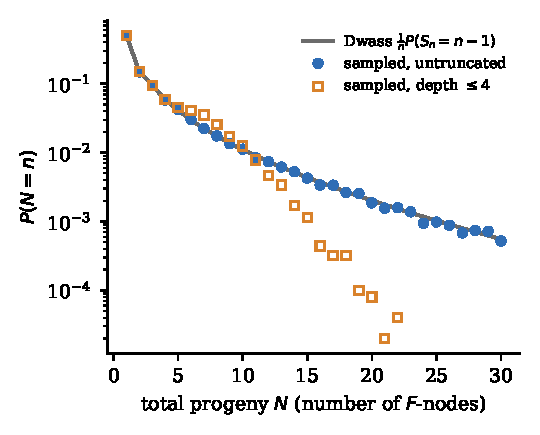
\includegraphics[width=\linewidth]{step01_progeny.pdf}\\(a)\end{minipage}\hfill
\begin{minipage}{0.49\linewidth}\centering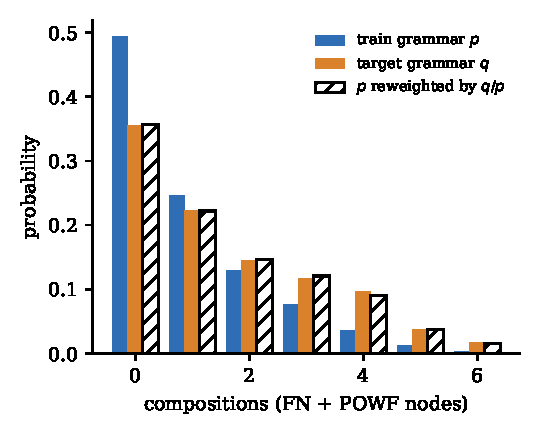
\includegraphics[width=\linewidth]{step01_shift.pdf}\\(b)\end{minipage}
\caption{(a) Law of the number of $F$-nodes: formula \eqref{eq:dwass} against the sampler. (b) Covariate shift between
two grammars, corrected by the exact likelihood ratio of Proposition~\ref{prop:expfam}.}\label{fig:step01}
\end{figure}

\paragraph{Exercises.}
\begin{exercise}
Show $\Var N=\sigma^2/(1-m)^3$ with $\sigma^2=\Var\xi$. (The test \code{test\_branching\_process\_mean\_progeny}
uses this to set its tolerance.)
\end{exercise}
\begin{exercise}
For i.i.d.\ $x_i\sim p$, show $\mathrm{ESS}/M\to1/\E_p[w^2]=1/(1+\chi^2(q\|p))$, and use
Proposition~\ref{prop:expfam} to write $\E_p[w^2]$ as a moment generating function of $c(x)$.
\end{exercise}

%=============================================================================
\section{Differentiation as structural recursion}
\label{sec:trace}
%=============================================================================

Before learning anything, we can \emph{measure} part of what makes a problem hard: the
procedure a student must carry out. Step 2 builds a differentiator that does what
a student does, one textbook rule at a time, and logs every rule it uses.

\paragraph{One clause per constructor.}
Trees are built from a few constructors (\code{Const}, \code{Var}, \code{Pow}, \code{Add},
\code{Mul}, \code{Div}, \code{Fn}). A function on trees defined by one clause per constructor,
calling itself only on immediate subtrees, is well defined by \emph{structural induction}:
the recursion terminates because every call is on a strictly smaller tree. Differentiation
is exactly such a function. Python's \code{match} statement lets the code read like the
definition:

\codefrom{src/calcdiff/solver\_trace.py}
\begin{lstlisting}
def _d(node, tr, depth, chain):
    def log(rule):                       # record "rule applied to node"
        tr.steps.append(Step(rule, node, depth, chain))
    def d(sub, *, through_chain=False):  # recurse one level down
        return _d(sub, tr, depth + 1, chain + through_chain)

    match node:
        case Pow(base, n):                       # (u^n)' = n u^(n-1) u'
            log("POWER")
            outer = _mul(Const(n), _pow(base, n - 1))
            if isinstance(base, Var):
                return outer
            log("CHAIN")
            return _mul(outer, d(base, through_chain=True))
        case Mul(factors):                       # (f1...fk)' = sum_i f_i' prod_{j!=i} f_j
            ...
            log("PRODUCT")
            terms = [_mul(*rest[:i], d(f), *rest[i+1:]) for i, f in enumerate(rest)]
            return _mul(c, _add(*terms))
        case Fn(name, arg):                      # g(u)' = g'(u) u'
            log(f"FN_{name}")
            outer = _fn_derivative(name, arg)
            ...
\end{lstlisting}
Read it as math. \code{d(sub)} is $D(\text{sub})$ one level deeper in the recursion. The flag
\code{through\_chain=True} marks that we passed \emph{inside} a composition, which is how
\code{chain\_depth} counts nested chain rules. \code{log} is a side effect that does not change the
value computed. The helpers \code{\_mul}, \code{\_add} do only the cleanup a person does
automatically ($1\cdot u=u$, $u+0=u$, multiply the constants together), so the output is the
derivative \emph{as a student would first write it}, unsimplified.

\paragraph{Why the rules compose: dual numbers.}
Let $\R[\varepsilon]=\R[t]/(t^2)$, so $\varepsilon^2=0$. For a polynomial, Taylor's theorem is exact:
$p(a+b\varepsilon)=p(a)+b\,p'(a)\varepsilon$. Use this to \emph{define} $g(a+b\varepsilon):=g(a)+b\,g'(a)\varepsilon$
for $g=\sin,\exp,\ldots$. Then
\[
(a+a'\varepsilon)(b+b'\varepsilon)=ab+(a'b+ab')\varepsilon,\qquad
g\bigl(u+u'\varepsilon\bigr)=g(u)+g'(u)\,u'\varepsilon,
\]
so the product rule is ring multiplication and the chain rule is composition. Formally,
evaluating a tree at $x+\varepsilon$ is a homomorphism from expressions into $\R[\varepsilon]$, and the
$\varepsilon$-coefficient is the derivative. Our recursion is the symbolic shadow of this, and the
numeric version is \emph{forward-mode automatic differentiation}. Every neural network in this
course is trained by computing gradients this way, or rather by its transpose, \emph{reverse mode}
(backpropagation), which we will meet in Section 11.

\paragraph{The trace is a measurement.}
For $\TExProblem$ the code returns
$\TExDerivative$ and the trace in Table~\ref{tab:trace}.
\emph{depth} is how many rule applications enclose this one (roughly, how much a student
must hold in working memory), and \emph{chain} is how many compositions we are inside.
From each trace we get a vector of counts $c(x)\in\mathbb N^{\text{rules}}$, the total
\code{n\_steps}, \code{max\_depth}, and \code{max\_chain\_depth}. These will become features in Section 3.

\begin{table}[h]\centering\footnotesize
\begin{tabular}{rccll}
\toprule
\# & depth & chain & rule & applied to \\
\midrule
1 & 0 & 0 & \code{PRODUCT} & $x^{2} \sin\left(e^{3 x}\right)$ \\
2 & 1 & 0 & \code{POWER} & $x^{2}$ \\
3 & 1 & 0 & \code{FN\_sin} & $\sin\left(e^{3 x}\right)$ \\
4 & 1 & 0 & \code{CHAIN} & $\sin\left(e^{3 x}\right)$ \\
5 & 2 & 1 & \code{FN\_exp} & $e^{3 x}$ \\
6 & 2 & 1 & \code{CHAIN} & $e^{3 x}$ \\
7 & 3 & 2 & \code{CONST\_MULT} & $3 x$ \\
8 & 4 & 2 & \code{VAR} & $x$ \\
\bottomrule
\end{tabular}

\caption{Trace of \code{derive} on $\TExProblem$, in the order the recursion visits nodes.}\label{tab:trace}
\end{table}

Over $\TNProblems$ generated problems, $\TFracChain$ need the chain rule, $\TFracProduct$ the product rule, and
$\TFracQuotient$ the quotient rule. $\TFracChainTwo$ have nested chains (\code{max\_chain\_depth} $\ge2$). The number of
steps has Spearman correlation $\TRhoNSteps$ with the grammar's derivation size $N$. That is
unsurprising, since both mostly measure size. Size is not difficulty, though: \code{n\_steps}
counts $\frac{d}{dx}5x^3$ and the inner $\frac{d}{dx}3x$ of $\sin(e^{3x})$ the same, even though only the
second is buried two compositions deep. Telling them apart is what features and learning are for.

\paragraph{Expression swell.}
Figure~\ref{fig:step02}(a) plots the size of the derivative against the size of the problem. A least-squares fit
on log-log axes has slope $\TSwellSlope$: derivatives grow faster than linearly. The product rule is to blame.
A product of $k$ factors of total size $n$ has a derivative with $k$ terms, each containing all
$k$ factors (one differentiated), so size $\Theta(kn)$, which is quadratic when the factors are small. The median
derivative is $\TMedSwell\times$ the problem's size, and the worst is $\TMaxSwell\times$. Swell is a real
component of difficulty, since a student has to write it all down without dropping a term.

\begin{figure}[h]\centering
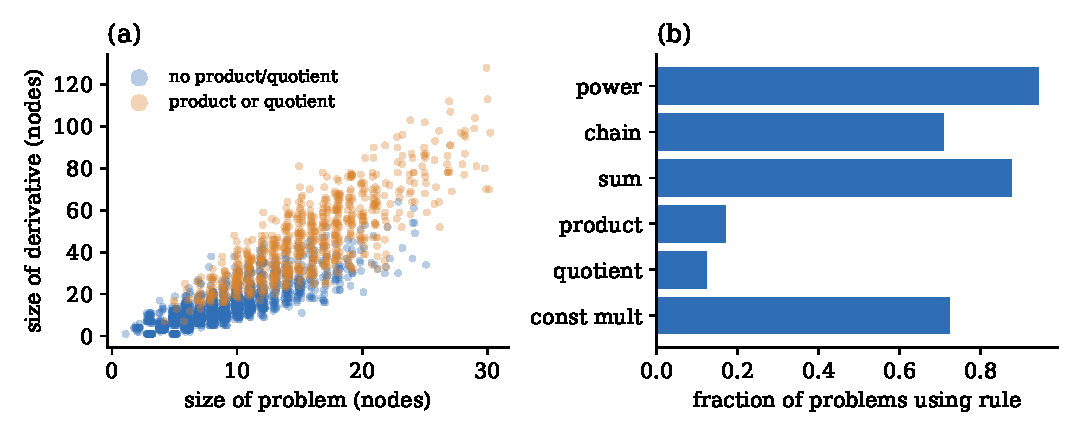
\includegraphics[width=0.92\linewidth]{step02_trace_stats.pdf}
\caption{(a) Expression swell: derivative size vs.\ problem size (jittered). (b) How often each rule is needed.}\label{fig:step02}
\end{figure}

\paragraph{Testing it: the identity theorem as a test oracle.}
How do we know \code{derive} is right? Comparing with \code{sympy.diff} symbolically
($\mathrm{simplify}(a-b)=0$) is slow and can fail to prove true identities. Instead, \code{numerically\_equal}
in \file{src/calcdiff/check.py} evaluates both at random points $z$ near the positive real axis, slightly
off it in $\mathbb C$:

\codefrom{src/calcdiff/check.py}
\begin{lstlisting}
z = rng.uniform(0.3, 2.5, n) + 1j * rng.uniform(-0.1, 0.1, n)
va, vb = fa(z), fb(z)                       # both sides, vectorized
ok = np.isfinite(va) & np.isfinite(vb)      # skip poles / overflow
return np.all(np.abs(va[ok] - vb[ok]) <= rtol * (1 + np.abs(vb[ok])))
\end{lstlisting}
Why is this a proof-quality test? Both sides are holomorphic on a connected open set $U$
(off poles and branch cuts). If $h=a-b\not\equiv0$ on $U$, its zeros are isolated by the identity theorem,
hence countable, hence of measure zero. A point drawn from a continuous distribution on
$U$ detects $h\neq0$ with probability 1 (in exact arithmetic, with a tolerance in floating point).
Complex points step off the branch cuts of $\ln$ and $\sqrt{\ }$, where real points can land on the wrong
side. Both sides use the same principal branches, and $\frac{d}{dz}\operatorname{Log}z=1/z$ holds off the cut.

\code{test\_matches\_sympy\_on\_generated\_problems} runs this on 500 problems. In the statistics run,
$\TNVerified$ of $\TNProblems$ agree, none disagree, and $\TNInconclusive$ are \emph{inconclusive}. Those are
problems like $e^{(x+9)^3}\approx e^{1000}$ that overflow double precision everywhere. Arbitrary precision does not
rescue them cheaply, since $\cos$ of a number near $10^{400}$ needs about 400 digits of $\pi$ just to reduce the
argument mod $2\pi$. So the checker honestly returns \code{None}. The generator found something too: $e^{(x^2+9)^5}$ is
legal but a bit absurd. We will see whether the instructor's labels penalize such problems.

\paragraph{Exercises.}
\begin{exercise}
Using only $\varepsilon^2=0$, derive the quotient rule from $(u+u'\varepsilon)/(v+v'\varepsilon)$.
(Why is $v+v'\varepsilon$ invertible in $\R[\varepsilon]$ exactly when $v\neq0$?)
\end{exercise}
\begin{exercise}
Let $P=f_1\cdots f_k$ with $|f_i|=s$ nodes each, and suppose each $|D f_i|\le\alpha s$. Bound $|D P|$ as produced by
\code{\_mul}/\code{\_add}, and show the bound is $\Theta(k^2s)$. What does this predict for the log-log slope in
Figure~\ref{fig:step02}(a), and why might the measured $\TSwellSlope$ be smaller?
\end{exercise}
\begin{exercise}
The random-point test can be fooled when $a-b$ vanishes on an open set, which cannot happen for a nonzero holomorphic function on a connected domain.
Give a pair of expressions whose difference is nonzero but vanishes on the entire sampling region
$\{0.3<\operatorname{Re}z<2.5,\ |\operatorname{Im}z|<0.1\}$ of the code. (Hint: think about $\sqrt{z^2}$ and the branch cut,
then about where that region sits.) Does this break our argument?
\end{exercise}

%=============================================================================
\section{Features: what the model is allowed to see}
\label{sec:features}
%=============================================================================

Every model until Section 11 sees a problem only through a \emph{feature map}
\[
  \varphi:\X\to\R^d,\qquad d=\FNFeatures,
\]
and a linear model predicts $f_\theta(x)=\theta\cdot\varphi(x)$. So the hypothesis class is
$\mathcal F=\{\theta\cdot\varphi:\theta\in\R^d\}$, a $d$-dimensional vector space of functions on $\X$,
spanned by the coordinate functions $\varphi_1,\dots,\varphi_d$. This is the cleanest way to say what
choosing features means: \textbf{you are choosing the subspace in which the answer must live}.
If the true difficulty $\delta$ is not close to that span, no amount of data will help (\emph{bias}).
If the span is large relative to the data, the fit is noisy (\emph{variance}). Section 8 makes that trade-off quantitative.

\paragraph{The code.} \code{featurize} assembles $\varphi(x)$ from three sources: the tree itself, the
trace from Section 2, and the derivative the student has to write down.

\codefrom{src/calcdiff/features.py}
\begin{lstlisting}
def featurize(tree: Node) -> np.ndarray:
    d, tr = derive(tree)                  # Step 2: derivative + trace
    c = tr.counts()                       # Counter: rule name -> times used
    pows = [n for n in walk(tree) if isinstance(n, Pow)]
    f = {
        "size": size(tree),
        "deriv_size": size(d),            # expression swell
        "n_chain": c["CHAIN"],
        "max_chain_depth": tr.max_chain_depth,
        "n_quotient": c["QUOTIENT"],
        "n_neg_exp": sum(p.exp < 0 for p in pows),
        "chain_in_product": _chains_under_product(tree, False),
        ...                               # 17 features in all
    }
    return np.array([f[name] for name in FEATURE_NAMES], dtype=float)
\end{lstlisting}
The dictionary-then-array pattern is deliberate. \code{FEATURE\_NAMES} fixes the coordinate order once,
so column $j$ of every matrix in the project means the same thing. For our running example
$\TExProblem$, Table~\ref{tab:phi} lists every coordinate. Check them against the trace in Table~\ref{tab:trace}.

\begin{table}[h]\centering\footnotesize
\begin{tabular}{lr@{\qquad}lr}
\toprule
\code{size} & 8 & \code{n\_const\_mult} & 1 \\
\code{depth} & 5 & \code{n\_trig} & 1 \\
\code{n\_terms} & 1 & \code{n\_exp} & 1 \\
\code{deriv\_size} & 22 & \code{n\_ln} & 0 \\
\code{n\_power} & 1 & \code{n\_sqrt} & 0 \\
\code{n\_chain} & 2 & \code{n\_neg\_exp} & 0 \\
\code{max\_chain\_depth} & 2 & \code{n\_frac\_exp} & 0 \\
\code{n\_product} & 1 & \code{chain\_in\_product} & 2 \\
\code{n\_quotient} & 0 &  &  \\
\bottomrule
\end{tabular}

\caption{$\varphi(x)$ for $x=\TExProblem$.}\label{tab:phi}
\end{table}

\paragraph{$\varphi$ is a quotient map, and that's a modeling claim.}
Any function of the form $\theta\cdot\varphi$ is constant on the fibers $\varphi^{-1}(v)$. So every
model we build until Section 11 asserts that \emph{problems with equal features are equally hard}. Among
$\FNProblems$ generated problems there are only $\FNDistinct$ distinct feature vectors. The largest fiber
has $\FBiggestClass$ problems (e.g.\ $\FTwinA$ and $\FTwinB$: fine, these really are equally hard). But
$\FCollideA$ and $\FCollideB$ also collide, because \code{n\_trig} lumps $\sin$, $\cos$ and $\tan$
together. An instructor might well say the cosine one is harder (that minus sign!). If so, our model
\emph{cannot} learn it: the information was discarded before learning began. Deciding which distinctions
to keep is the art of feature engineering, and it is where your teaching experience enters the model.

\paragraph{Interactions: what ``linear'' cannot do.}
A linear model is \emph{additive}: the effect of one more chain rule is the same $\theta_{\text{chain}}$ whether or not
there is a product around it. If you believe a chain rule \emph{inside} a product rule is harder than the
two separately (the student must hold $u'v+uv'$ open while doing a chain rule inside it), the model can only
express that through a feature equal to that interaction:

\codefrom{src/calcdiff/features.py}
\begin{lstlisting}
def _chains_under_product(node: Node, under: bool) -> int:
    here = int(under and _is_chain(node))      # a chain rule with a product above it?
    under = under or (isinstance(node, (Mul, Div)) and _has_two_nonconst(node))
    return here + sum(_chains_under_product(ch, under) for ch in node.children())
\end{lstlisting}
This is another structural recursion, like Section 2, but now the flag \code{under} is \emph{inherited}
downward: once we pass through a product or quotient (a genuine one, not $5\cdot u$), every chain rule below
it counts. Hand-built interactions do not scale (there are $\binom{d}{2}$ pairs). Gradient-boosted trees (Section 9) and
neural networks (Section 11) are, in large part, machines for discovering interactions automatically.

\paragraph{Geometry of the feature matrix.}
Stack the features of $n$ problems into $\Phi\in\R^{n\times d}$. Figure~\ref{fig:step03}(a) shows the correlations
over $\FNProblems$ problems. Several features nearly duplicate each other: $\FTopPairA$ and $\FTopPairB$ have
correlation $\FTopCorr$, and \code{size} with \code{n\_power} has $\FCorrSizePower$. The spectrum of the correlation
matrix, panel (b), shows how close $\Phi$ is to rank-deficient. The eigenvalues run from $\FEigMax$ down to $\FEigMin$
(condition number $\approx\FCond$), and the two smallest eigenvectors are essentially
``\code{size} $\approx$ a combination of the rule counts'' and ``\code{deriv\_size} $\approx$ a combination of the rule counts''.

Why care? For least squares with noise variance $\sigma^2$, $\operatorname{Cov}(\hat\theta)=\sigma^2(\Phi^\top\Phi)^{-1}$. Along the
eigenvector $v_i$ of $\Phi^\top\Phi$ with eigenvalue $\lambda_i$, $\Var(v_i\cdot\hat\theta)=\sigma^2/\lambda_i$. Directions
with tiny $\lambda_i$ are directions in which the data barely constrain $\theta$. The individual weights on \code{size} and the
rule counts will swing wildly from sample to sample, even though their combined prediction is stable.
(Section 4 shows that Bradley--Terry has exactly this structure, with $\Phi^\top\Phi$ replaced by a weighted version.)
Two standard fixes, both coming in Section 6:
drop redundant features, or add a ridge penalty $\tfrac\lambda2\|\theta\|^2$, which replaces $\lambda_i$ by $\lambda_i+\lambda$
and caps every variance at $\sigma^2/\lambda$.

\begin{figure}[h]\centering
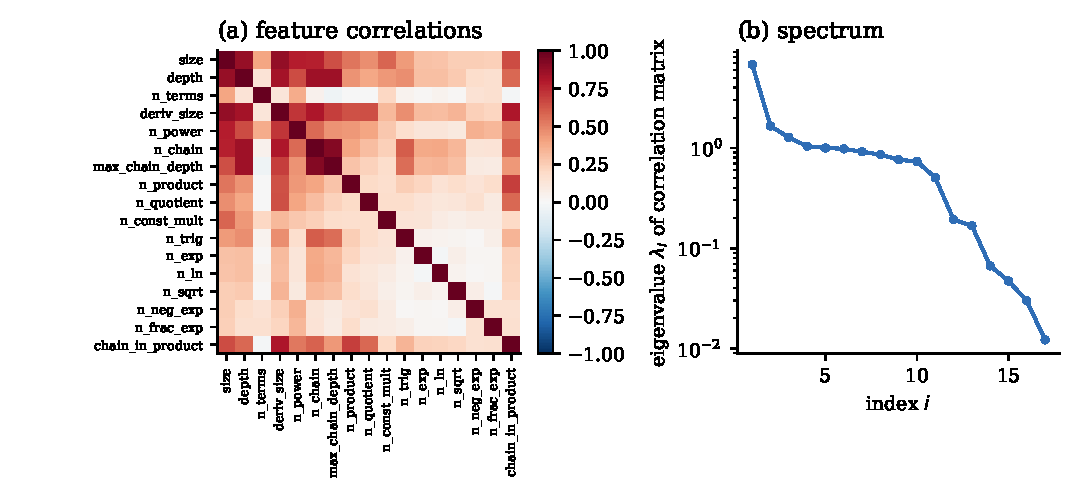
\includegraphics[width=0.92\linewidth]{step03_features.pdf}
\caption{(a) Correlations among the $\FNFeatures$ features on $\FNProblems$ generated problems. (b) Eigenvalues of
the correlation matrix (log scale). The last few are what make individual weights unstable.}\label{fig:step03}
\end{figure}

\paragraph{Standardization, and the first appearance of leakage.}
A ridge penalty is not invariant under rescaling a feature. Measuring \code{size} in nodes (mean $\approx 10$)
while \code{n\_quotient} is mostly 0 or 1 would quietly penalize them very differently (Exercise~\ref{ex:scale}).
The standard fix is $z_j=(\varphi_j-\mu_j)/s_j$:

\codefrom{src/calcdiff/features.py}
\begin{lstlisting}
class Standardizer:
    def fit(self, X):
        self.mean_ = X.mean(axis=0)
        sd = X.std(axis=0)
        self.std_ = np.where(sd > 0, sd, 1.0)   # a constant column stays constant
        return self
    def transform(self, X):
        return (X - self.mean_) / self.std_
\end{lstlisting}
The split into \code{fit} and \code{transform} is the important design point. $\mu$ and $s$ are \emph{parameters
estimated from data}, so they must be fit on training problems only and then applied, frozen, to test problems.
Computing them on everything lets test data influence training, which is called \emph{leakage}. It is a small effect here,
and a fatal one in many real projects. Section 5 is about this.

\paragraph{Exercises.}
\begin{exercise}\label{ex:scale}
Show that minimizing $\widehat R(\theta)+\frac\lambda2\|\theta\|^2$ with feature $\varphi_j$ replaced by $c\,\varphi_j$ is equivalent to
the original problem with the penalty on $\theta_j$ changed from $\frac\lambda2\theta_j^2$ to $\frac{\lambda}{2c^2}\theta_j^2$. Which features does
an unstandardized ridge penalize most?
\end{exercise}
\begin{exercise}
Propose one feature that would separate $\FCollideA$ from $\FCollideB$, and one that captures ``the answer needs
simplification''. Write each as a structural recursion like \code{\_chains\_under\_product}. Which of your
features are invariant under reordering the terms of a sum? Should they be?
\end{exercise}

%=============================================================================
\section{Bradley--Terry: the first actual learning}
\label{sec:bt}
%=============================================================================

Now we fit the model \eqref{eq:bt} to comparisons. In this section each problem $i\in\{1,\dots,n\}$
gets its own free parameter $\theta_i$, with no features yet. This is the classical estimation problem,
and almost everything about the feature-based model of Section 6 already shows up here.

\paragraph{The likelihood, as logistic regression on differences.}
Comparison $k$ involves items $(i_k,j_k)$ with label $y_k=1$ if $i_k$ was judged harder. Put $s_k=2y_k-1\in\{\pm1\}$
and $t_k=\theta_{i_k}-\theta_{j_k}$. Since $1-\sigma(t)=\sigma(-t)$, both outcomes have likelihood $\sigma(s_kt_k)$, and the
negative log-likelihood is
\begin{equation}\label{eq:nll}
  L(\theta)=\sum_k\log\bigl(1+e^{-s_kt_k}\bigr)+\tfrac\lambda2\|\theta\|^2,\qquad t=D\theta,
\end{equation}
where $D$ is the $m\times n$ \emph{design matrix} with rows $e_{i_k}-e_{j_k}$. That is all logistic regression is: a
linear map followed by $u\mapsto\log(1+e^{-u})$ (\emph{softplus}). In Section 6 we will simply replace the rows
$e_i-e_j$ by $\varphi(x_i)-\varphi(x_j)$, and every line of code below carries over unchanged.

\codefrom{src/calcdiff/models/bt.py}
\begin{lstlisting}
def one_hot_design(pairs, n_items):
    D = np.zeros((len(pairs), n_items))
    rows = np.arange(len(pairs))
    D[rows, pairs[:, 0]] = 1.0            # +e_i
    D[rows, pairs[:, 1]] = -1.0           # -e_j
    return D

def nll(theta, D, y, l2=0.0):
    t = D @ theta
    # cross-entropy: softplus(t) - y t
    return float((np.logaddexp(0.0, t) - y * t).sum() + 0.5 * l2 * theta @ theta)
\end{lstlisting}
The code uses the equivalent form $\log(1+e^{t_k})-y_kt_k$ (the \emph{cross-entropy} between $y_k$ and $\sigma(t_k)$). For
$y_k\in\{0,1\}$ it equals the summand in \eqref{eq:nll}, and it also makes sense for $y_k=\frac12$, which Section 7 needs for ties.
\code{np.logaddexp(0, u)} computes $\log(e^0+e^u)=\log(1+e^u)$ without ever forming $e^u$. The naive
\code{np.log(1 + np.exp(u))} overflows to \code{inf} for $u>710$, which happens as soon as a fit grows confident.
Numerical care like this is a large part of practical ML.

\paragraph{Gradient and Hessian.}
With $p=\sigma(D\theta)$ and $W=\operatorname{diag}\bigl(p(1-p)\bigr)$, a short computation using $\sigma'=\sigma(1-\sigma)$ gives
\[
  \nabla L=D^\top(p-y)+\lambda\theta,\qquad \nabla^2L=D^\top WD+\lambda I.
\]
The gradient has a nice reading: each comparison pushes its two items apart by ``predicted minus observed''.

\codefrom{src/calcdiff/models/bt.py}
\begin{lstlisting}
def grad_hess(theta, D, y, l2=0.0):
    p = expit(D @ theta)                                   # sigma, elementwise
    g = D.T @ (p - y) + l2 * theta
    H = (D * (p * (1 - p))[:, None]).T @ D + l2 * np.eye(len(theta))
    return g, H
\end{lstlisting}
\code{D * w[:, None]} scales row $k$ of $D$ by $w_k$ via broadcasting, so the last line is $D^\top WD$ without
building the $m\times m$ matrix $W$. A test (\code{test\_gradient\_matches\_finite\_differences}) checks $\nabla L$
against central differences. Always do this when you hand-derive a gradient.

\paragraph{The Hessian is a graph Laplacian.}
Expand $D^\top WD=\sum_kw_k(e_{i_k}-e_{j_k})(e_{i_k}-e_{j_k})^\top$. This is the Laplacian $L_w$ of the
\emph{comparison graph} $G$ on the items, with an edge of weight $w_k=p_k(1-p_k)$ for each comparison. Its quadratic form is
\[
  v^\top L_wv=\sum_kw_k\,(v_{i_k}-v_{j_k})^2\ \ge0 .
\]
So $L$ is convex, and $v^\top L_wv=0$ iff $v$ is constant on each connected component of $G$ (all $w_k>0$).
Two consequences:
\begin{itemize}[nosep]
\item \textbf{Identifiability.} If $G$ is connected, $\ker L_w=\operatorname{span}(\mathbf 1)$: the data pin down $\theta$
  up to exactly one additive constant, as promised in Section 0. If $G$ has two components, each one floats
  independently, and comparing items across them is meaningless.
\item \textbf{The gauge is preserved automatically.} For singular $H$, the least-squares solver
  used in \code{fit\_newton} returns the minimum-norm solution of $H\,\Delta=-g$, which lies in
  $\operatorname{range}(H)=\mathbf 1^\perp$. Starting at $\theta=0$, every iterate satisfies $\sum_i\theta_i=0$.
\end{itemize}
The test \code{test\_hessian\_is\_weighted\_graph\_laplacian} checks all of this numerically: symmetric,
rows summing to 0, off-diagonals $\le0$, and exactly one zero eigenvalue.

\paragraph{Does a maximizer exist? Zermelo's condition.}
Convexity gives uniqueness (on $\mathbf 1^\perp$), but not existence. Suppose a set $S$ of items never \emph{lost} to an item
outside $S$. Then adding $c>0$ to every $\theta_i$, $i\in S$, increases every cross-term $s_kt_k$, so the loss strictly
decreases for all $c$ and the infimum is not attained. The converse holds as well:

\begin{theorem}[Zermelo 1929; Ford 1957]
With $\lambda=0$, $L$ has a minimizer (unique on $\mathbf 1^\perp$) iff the directed graph with an edge
winner$\to$loser for each comparison is strongly connected.
\end{theorem}

\codefrom{src/calcdiff/models/bt.py}
\begin{lstlisting}
def mle_exists(pairs, y, n_items):
    win = np.where(y[:, None] == 1, pairs, pairs[:, ::-1])   # rows (winner, loser)
    G = coo_matrix((np.ones(len(win)), (win[:, 0], win[:, 1])), shape=(n_items, n_items))
    n_comp, _ = connected_components(G, directed=True, connection="strong")
    return n_comp == 1
\end{lstlisting}
This is not a corner case. In the very first test I wrote, with 30 items and about 40 comparisons each, one item
(true $\delta=-3.3$) lost all of its games, and Newton happily drove $\theta$ for that item past $-27$. Worse, it then reported
\emph{convergence}: along the escape ray the gradient tends to 0, so a gradient-based stopping rule is fooled. The test
\code{test\_perfect\_separation\_diverges\_without\_ridge} pins this behavior down. With $n=\BNItems$ items, Experiment C
below found a finite MLE in a fraction $\BExistsThirtyTwo$ of the datasets with 32 comparisons per item. The more items, the more chances
that \emph{some} item goes undefeated or winless.

\paragraph{The fix: ridge = MAP with a Gaussian prior.}
Put a prior $\theta_i\overset{\text{iid}}\sim N(0,1/\lambda)$. The negative log-posterior is \eqref{eq:nll} with the
$\frac\lambda2\|\theta\|^2$ term, which is strictly convex and coercive, so the \emph{maximum a posteriori} (MAP) estimate always exists
and is unique. We use $\lambda=\BLTwo$ (prior sd $\BPriorSD$ logits, very weak) from now on. A pleasant fact (Exercise~\ref{ex:gauge}):
because every row of $D$ sums to zero, the ridge optimum satisfies $\sum_i\theta_i=0$ exactly. In the experiment
below, $|\sum_i\hat\theta_i|=\BSumTheta$.

\paragraph{Optimization: Newton vs.\ gradient descent.}
Newton's method minimizes the local quadratic model $L(\theta)+g^\top\Delta+\frac12\Delta^\top H\Delta$, giving
$\Delta=-H^{-1}g$:

\codefrom{src/calcdiff/models/bt.py}
\begin{lstlisting}
for it in range(1, max_iter + 1):
    g, H = grad_hess(theta, D, y, l2)
    step = np.linalg.lstsq(H, -g, rcond=None)[0]     # solve H step = -g
    decrement = float(-g @ step)                      # Newton decrement g^T H^-1 g
    if decrement / 2 < tol:                           # ~ L(theta) - L*
        return BTFit(theta, it - 1, True, hist, H)
    t = 1.0
    while nll(theta + t * step, D, y, l2) > hist[-1] - 0.25 * t * decrement:
        t *= 0.5                                      # backtrack until enough decrease
    theta = theta + t * step
\end{lstlisting}
Two details. The quantity $\lambda^2=g^\top H^{-1}g$ (the \emph{Newton decrement}) is the decrease the quadratic model predicts.
Half of it estimates the optimality gap $L(\theta)-L^\ast$, which makes it a principled, scale-free stopping rule. And
the \code{while} loop is an Armijo backtracking line search: far from the optimum the quadratic model can be wrong, so we halve
the step until the actual decrease is at least a quarter of the predicted one. Near the optimum $t=1$ is accepted
and convergence is \emph{quadratic} (the number of correct digits doubles each step).

Gradient descent instead takes $\theta\leftarrow\theta-\eta\nabla L$ with $\eta=1/\beta$, where
$\beta=\|D\|_2^2/4+\lambda\ge\lambda_{\max}(H)$ since $p(1-p)\le\frac14$. For a $\mu$-strongly convex, $\beta$-smooth function it
converges \emph{linearly}: $L(\theta_t)-L^\ast\le(1-\mu/\beta)^t(L(\theta_0)-L^\ast)$. Figure~\ref{fig:step04}(b) shows
the difference: Newton needs $\BNewtonIters$ iterations, while gradient descent needs $\BGDToTen$ to reach a gap of $10^{-10}$
(the Hessian at the optimum has condition number $\BHessCond$). Why does all of deep learning use gradient methods anyway? A Newton step
costs $O(d^3)$, and $d=10^9$ is common. Here $d=\BNItems$, so Newton is the right tool.

\paragraph{Uncertainty: Fisher information and effective resistance.}
Near the optimum the log-posterior is approximately quadratic, so the posterior is approximately
$N(\hat\theta,H^{-1})$ (the \emph{Laplace approximation}). The frequentist twin is asymptotic normality,
$\hat\theta\approx N(\theta^\ast,\mathcal I^{-1})$, with the Fisher information $\mathcal I=\E[D^\top WD]$. For a difference of two items,
\[
  \Var(\hat\theta_i-\hat\theta_j)\approx(e_i-e_j)^\top L_w^{+}(e_i-e_j)=R_{\mathrm{eff}}(i,j),
\]
the \emph{effective resistance} between $i$ and $j$ in the electrical network with conductance $w_k$ on each comparison edge.
That gives two design lessons for later. Many parallel paths of comparisons lower the variance, just as parallel resistors do. And each comparison's
conductance is $w=\sigma'(\delta_i-\delta_j)\le\frac14$, maximal for \emph{evenly matched} pairs and exponentially small for
lopsided ones. Comparing $x^2$ with a monster problem teaches us almost nothing. This is the seed of active learning (Section 10).

\begin{remark}[a bug that was really a lesson]
My first version of Experiment C predicted an RMSE of $0.33$ from the Fisher information, while the simulation
achieved $0.24$. The theory was beating reality! The culprit was the direction $\mathbf 1$. The data have no
curvature there, so $H^{-1}$ assigns it the pure prior variance $1/\lambda=10$, which adds $10/n$ to every
diagonal entry. But $\hat\theta\perp\mathbf 1$ exactly, so there is never any error in that direction. The right covariance is
$PH^{-1}P$ with $P=I-\frac1n\mathbf 1\mathbf 1^\top$ (\code{covariance(centered=True)}), and with it theory and
simulation agree. The naive mean standard error was $\BMeanSENaive$, and the corrected one is $\BMeanSE$.
\end{remark}

\paragraph{Experiments on a planted truth.}
\file{src/calcdiff/synthetic.py} defines a simulated instructor: $\delta(x)=w\cdot\varphi(x)+\tau\varepsilon(x)$, with
hand-picked weights $w$ (e.g.\ $0.55$ logits per quotient rule) and an idiosyncratic part $\tau=0.5$ that the
features cannot see. It then answers comparisons by sampling from \eqref{eq:bt}. My first weights gave $\delta$ a spread
of 10 logits, and only about 10\% of random datasets with 40 comparisons per item satisfied Zermelo's condition. The extremes simply never lost. Scaling the weights
down gave sd $\BDeltaSD$ and range $[\BDeltaMin,\BDeltaMax]$. On $\BNItems$ problems with $\BM$ random comparisons
($\BPerItem$ per item), Figure~\ref{fig:step04}:
\begin{enumerate}[nosep,label=(\alph*)]
\item \textbf{Recovery.} RMSE $\BRMSE$ logits, Spearman $\rho=\BSpearman$ with the truth, and $\BCoverage\%$ of the
  nominal 95\% intervals $\hat\theta_i\pm1.96\,\mathrm{se}_i$ contain $\delta_i$. Note the error bars widen at the
  extremes: lopsided comparisons carry little information.
\item \textbf{Optimization.} Newton converges quadratically, while gradient descent converges linearly.
\item \textbf{Rate.} RMSE against comparisons per item $k$, averaged over 5 datasets. The log-log slope is $\BRateSlope$,
  matching the $k^{-1/2}$ predicted by $\mathcal I\propto k$. The dashed Fisher curve is computed from the truth with no fitting,
  and it lands on the simulation ($\BLargeKRMSE$ vs.\ $\BLargeKTheory$ at $k=128$). At $k=2$ the prior dominates: the
  estimates barely leave 0, so the RMSE ($\BSmallKRMSE$) is close to the spread of $\delta$ itself ($\BDeltaSD$).
\end{enumerate}

\begin{figure}[h]\centering
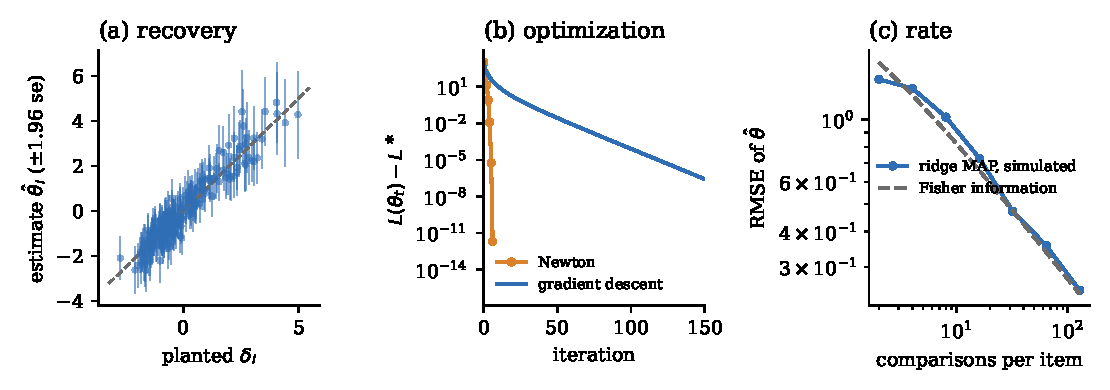
\includegraphics[width=\linewidth]{step04_bt.pdf}
\caption{Bradley--Terry on synthetic data. (a) Estimates vs.\ planted difficulty with 95\% intervals.
(b) Optimality gap per iteration. (c) Error vs.\ comparisons per item, against the Fisher-information prediction.}\label{fig:step04}
\end{figure}

\paragraph{What this model cannot do.}
Item-level BT has nothing to say about problem $n+1$: it has no parameter for it. And it needs on the order of $k\approx40$
comparisons \emph{per problem} for $\pm0.5$-logit accuracy, which is far beyond any instructor's patience for a large bank. Section 6
replaces $e_i$ by $\varphi(x_i)$. The number of parameters drops from $n$ to $d=\FNFeatures$, and information is
\emph{shared}: a comparison involving one quotient problem teaches the model about all quotient problems.

\paragraph{Exercises.}
\begin{exercise}\label{ex:gauge}
Show that for one-hot $D$ and $\lambda>0$, the minimizer of \eqref{eq:nll} satisfies $\mathbf 1^\top\hat\theta=0$.
(Hint: $D\mathbf 1=0$. Take the inner product of the stationarity equation with $\mathbf 1$.)
\end{exercise}
\begin{exercise}
Items $1,\dots,n$ compared only along a path ($1$ vs.\ $2$, $2$ vs.\ $3$, \dots), each pair $r$ times, all with $w=\frac14$.
Compute $\Var(\hat\theta_1-\hat\theta_n)$ via effective resistance, and compare with the complete graph using the same
total number of comparisons. What does this say about how to schedule an instructor's comparisons?
\end{exercise}
\begin{exercise}
Prove the ``only if'' direction of Zermelo's theorem carefully. Then explain why it implies that the maximum likelihood
estimate fails to exist with probability tending to 1 if $n\to\infty$ with $k$ fixed.
\end{exercise}

%=============================================================================
\section{Evaluation: what does ``good'' mean?}
\label{sec:eval}
%=============================================================================

A model is only as trustworthy as the experiment that evaluates it. This section builds
that experiment before we have a model worth evaluating, so that we can't tune the experiment to flatter the model.

\paragraph{Hold out problems, not comparisons.}
The deployed model will score problems \emph{nobody has compared}. So the target is
\[
  R=\E_{x,x'\sim\mathcal D}\ \E_{y\mid x,x'}\,\ell\bigl(\hat\delta(x)-\hat\delta(x'),\,y\bigr),
  \qquad x,x'\ \text{independent of the training problems.}
\]
The independent unit, the thing that is exchangeable, is the \emph{problem}. If we split
comparisons at random, the same problems sit on both sides of the split, and we measure interpolation among problems we
have already seen. That is \emph{leakage}: information about the test set reaching the model through the back door.
Table~\ref{tab:split} makes it concrete. Item-level BT from Section 4 looks excellent on new
comparisons among problems it has seen, and is a coin flip on unseen problems, because it has nothing to say about them.

\begin{table}[h]\centering\small
\begin{tabular}{llcc}
\toprule
model & evaluated on & accuracy & oracle ceiling \\
\midrule
item-level BT & new pairs, seen problems & 0.733 & 0.760 \\
item-level BT & unseen problems & 0.500 & 0.774 \\
feature BT & new pairs, seen problems & 0.733 & 0.760 \\
feature BT & unseen problems & 0.747 & 0.774 \\
\bottomrule
\end{tabular}

\caption{The same two models under two evaluation protocols (synthetic instructor; 200 training problems, 200 unseen).}\label{tab:split}
\end{table}

\paragraph{Metrics.}
\begin{itemize}[nosep]
\item \emph{Pairwise accuracy}: the fraction of decided comparisons ordered correctly by the scores.
  If every pair were labeled by the true order, accuracy would be exactly $(1+\tau)/2$ with $\tau$ Kendall's tau (Exercise~\ref{ex:tau}).
\item \emph{Log-loss}: the mean cross-entropy $\frac1m\sum_k[\log(1+e^{t_k})-y_kt_k]$. It is a \emph{proper scoring rule}:
  its expectation is minimized by reporting the true probability (Gibbs' inequality). So it rewards calibrated
  confidence, not just the right order. We use it to \emph{tune} and accuracy to \emph{report}.
\item \emph{Rank correlation} with the truth (Spearman's $\rho$, Kendall's $\tau$). This is only available on synthetic data.
\end{itemize}

\codefrom{src/calcdiff/evaluate.py}
\begin{lstlisting}
def pairwise_accuracy(scores, pairs, y, weights=None):
    decided = y != 0.5                              # skip "about the same"
    diff = scores[pairs[:, 0]] - scores[pairs[:, 1]]
    tied = np.abs(diff) < 1e-9                      # equal scores, up to float dust
    credit = np.where(tied, 0.5, ((diff > 0) == (y == 1)).astype(float))
    w = np.ones(len(y)) if weights is None else weights
    w = w * decided
    return float((w * credit).sum() / w.sum())
\end{lstlisting}
Two conventions matter. A model that refuses to choose (equal scores) gets half credit, so a constant model
scores \emph{exactly} $0.5$. And the tolerance \code{1e-9} is not cosmetic. My first run reported $0.492$ for item-level BT on unseen
problems, where every score is $0$. The $\theta$'s were $\pm10^{-17}$ rather than exactly zero, so ties were being broken at random.
The optional \code{weights} argument is for the bootstrap below.

\paragraph{The noise ceiling.}
Labels are random: even a perfect model is right on a comparison only with probability $\max(p,1-p)$, where
$p=\sigma(\delta_i-\delta_j)$. So no model can beat $C=\E\max(p,1-p)$ (\code{bayes\_ceiling}), and how close we get matters more
than the raw number. Figure~\ref{fig:step05} shows $C$ as a function of the spread of difficulty. If $\delta\sim N(0,s^2)$, then
$C=\E\,\sigma(|\sqrt2\,sZ|)$. For our simulated instructor (sd $\EDeltaSD$), $C\approx\ECeilHere$. An instructor whose judgments vary
less (a smaller spread) caps every model lower. Section 7 shows how to estimate your own ceiling from repeated pairs.

\begin{figure}[h]\centering
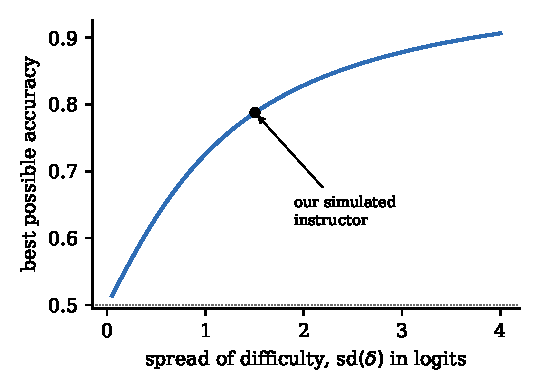
\includegraphics[width=0.48\linewidth]{step05_ceiling.pdf}
\caption{Best achievable pairwise accuracy as a function of how spread out the true difficulties are.}\label{fig:step05}
\end{figure}

\paragraph{Error bars when comparisons share problems.}
On the $\ENTest$ unseen problems, the feature model of Section 6 scores accuracy $\EFeatAcc$ on $\ENTestPairs$ comparisons. The
textbook binomial interval is $\pm1.96\sqrt{a(1-a)/m}=\pm\ENaiveHalf$, and it is wrong. The comparisons are not independent:
every comparison involving a problem the model misjudges tends to be wrong together. Accuracy is (essentially)
a \emph{U-statistic} $U=\binom n2^{-1}\sum_{i<j}h(x_i,x_j)$ in the problems, and Hoeffding's decomposition gives
\[
  \Var U=\frac{4\zeta_1}{n}+O(n^{-2}),\qquad \zeta_1=\Var_x\bigl(\E[h(x,x')\mid x]\bigr).
\]
The precision is governed by the number of \emph{problems} $n$, not the number of comparisons $m$. Once $m\gg n$, more comparisons
among the same problems barely help. The fix is to resample problems:

\codefrom{src/calcdiff/evaluate.py}
\begin{lstlisting}
for _ in range(n_boot):
    draw = rng.choice(items, size=len(items), replace=True)   # resample PROBLEMS
    c = np.bincount(draw, minlength=n).astype(float)           # multiplicity c_i
    w = c[pairs[:, 0]] * c[pairs[:, 1]]                        # comparison weight c_i c_j
    stats.append(metric(w))
\end{lstlisting}
If problem $i$ is drawn $c_i$ times, each comparison $(i,j)$ appears $c_ic_j$ times among the resampled problems, and the metric is
recomputed with those weights. The result is $[\EBootLo,\EBootHi]$, a half-width of $\EBootHalf$, which is $\EWidthRatio\times$ the naive one.
On real data with a few hundred problems, this is the error bar to believe.

\paragraph{Exercises.}
\begin{exercise}\label{ex:tau}
Suppose every pair $\{i,j\}$ is labeled once by the true order ($y=\mathbf 1[\delta_i>\delta_j]$, no ties). Show that the pairwise accuracy of scores $s$ equals $(1+\tau(s,\delta))/2$.
\end{exercise}
\begin{exercise}
Show that $q\mapsto\E_{y\sim\mathrm{Bern}(p)}[-y\log q-(1-y)\log(1-q)]$ is uniquely minimized at $q=p$, and that accuracy (as a function of reported $q$) is not strictly proper.
\end{exercise}
\begin{exercise}
For the U-statistic above, derive $\Var U=\binom n2^{-1}\bigl(2(n-2)\zeta_1+\zeta_2\bigr)$, where $\zeta_2=\Var h$. When $m$ comparisons are sampled at random instead of all $\binom n2$, what extra term appears?
\end{exercise}

%=============================================================================
\section{Linear Bradley--Terry on features: generalizing to new problems}
\label{sec:featbt}
%=============================================================================

Now we combine Sections 3 and 4. Difficulty is a linear function of standardized features,
\[
  \hat\delta(x)=\theta\cdot z(x),\qquad \P(x_i\succ x_j)=\sigma\bigl(\theta\cdot(z_i-z_j)\bigr),
\]
so the design matrix has rows $z_i-z_j\in\R^{d}$ instead of $e_i-e_j\in\R^n$. It is the same convex problem, with the same
gradient, Hessian and Newton iteration. \code{fit\_newton} is reused without changing a character. (No intercept:
it would cancel in every difference.)

\codefrom{src/calcdiff/models/feature\_bt.py}
\begin{lstlisting}
def fit(self, Phi, pairs, y):
    X = self._select(Phi)                       # all features, or a subset for baselines
    seen = np.unique(pairs)                     # problems in TRAINING comparisons only
    self.scaler_ = Standardizer().fit(X[seen])  # no leakage from held-out problems
    Z = self.scaler_.transform(X)
    D = Z[pairs[:, 0]] - Z[pairs[:, 1]]         # rows z_i - z_j
    self.fit_ = fit_newton(D, y, l2=self.l2)
    self.theta_ = self.fit_.theta
    return self

def score(self, Phi):                           # works for ANY problem
    return self.scaler_.transform(self._select(Phi)) @ self.theta_
\end{lstlisting}
\code{Phi} holds features for every problem, both labeled and not. \code{pairs} index into its rows. \code{score} is where the
generalization happens: it never asks whether a problem was ever compared.

\paragraph{Why so few labels suffice: shared information.}
The Fisher information is now $\sum_kw_k(z_{i_k}-z_{j_k})(z_{i_k}-z_{j_k})^\top$, a $d\times d$ matrix with $d=\FNFeatures$, instead of the $n\times n$ Laplacian.
Every comparison informs \emph{all} problems through $\theta$: a comparison involving one quotient problem teaches the
model something about every quotient problem. The variance of a prediction for a brand-new problem $x$ is $z(x)^\top H^{-1}z(x)$,
which shrinks like $1/m$ no matter whether $x$ was ever seen. This is the payoff of the restriction we accepted in Section 3. We gave up
the ability to tell apart problems with equal features, and in exchange $d$ parameters replace $n$.

\paragraph{Results.}
Figure~\ref{fig:step06}(a) trains on $m$ random comparisons among $\GNTrainProblems$ problems and tests on $\GNTestProblems$ \emph{unseen} ones
(8 repetitions per $m$; bands are $\pm1$ sd).
\begin{itemize}[nosep]
\item Two ceilings: the oracle ($\GCeiling$) knows the idiosyncratic part $\tau\varepsilon$ of the planted difficulty, which no
  feature model can see, while the planted feature part $w\cdot\varphi$ scores $\GFeatCeiling$. The gap between them is irreducible
  \emph{for this feature set}. Only better features can close it.
\item With $m=200$ comparisons (about $\GPerProblemAtTwoHundred$ per training problem) the model is within one point of the feature
  ceiling ($\GAccTwoHundred$). Compare the $\approx40$ comparisons \emph{per problem} item-level BT needed in Section 4.
\item Baselines: \code{size} alone plateaus at $\GSizeOnlyLarge$. \code{deriv\_size} alone reaches $\GDerivOnlyLarge$, almost as good as all
  17 features. In this synthetic world ``bigger derivative = harder'' is a strong proxy, because the planted weights mostly
  reward things that also make the derivative bigger. Whether that is true of \emph{your} judgments is an empirical question,
  and one of the first things we will check with real labels.
\end{itemize}

\paragraph{Reading the weights.}
Panel (b) compares learned and planted weights in \emph{raw} units (logits per unit of feature). Since $z_j=(\varphi_j-\mu_j)/s_j$,
$\theta\cdot z=\sum_j(\theta_j/s_j)\varphi_j+\text{const}$, so the raw weight is $\theta_j/s_j$ (\code{raw\_weights}).

How sure are we of each weight? The Laplace standard error $\sqrt{(H^{-1})_{jj}}/s_j$ gives intervals that contain $\GCovered$ of the $\GNFeat$ planted weights,
fewer than the $\approx16$ that nominal 95\% coverage would suggest. Two separate things go wrong, and they are worth telling apart.
\begin{itemize}[nosep]
\item \textbf{The standard errors are too small.} Laplace assumes the comparisons are independent. But the planted difficulty has a
  per-problem part $\tau\varepsilon(x)$, invisible to the features and shared by \emph{every} comparison involving $x$. This is the dependence of Section 5 again, now
  hurting the \emph{weights} rather than the accuracy, and the cure is the same: resample problems and refit.

\codefrom{src/calcdiff/models/feature\_bt.py}
\begin{lstlisting}
def problem_bootstrap(Phi, pairs, y, l2, rng, n_boot=200):
    for _ in range(n_boot):
        c = np.bincount(rng.choice(items, size=len(items), replace=True), minlength=n)
        idx = np.repeat(np.arange(len(pairs)), c[pairs[:, 0]] * c[pairs[:, 1]])
        out.append(FeatureBT(l2=l2).fit(Phi, pairs[idx], y[idx]).raw_weights())
\end{lstlisting}
  Here the bootstrap standard errors are $\GSERatio\times$ larger (median). Over 6 independent replications with light ridge, Laplace intervals covered
  $\GRepCovLaplace\%$ of planted weights, and problem-bootstrap intervals $\GRepCovBoot\%$, with standard errors $\GRepSERatio\times$ larger.
  (An earlier version of these notes reported all 17 covered. That was luck.)
\item \textbf{Ridge is biased, and a standard error cannot see bias.} Even the bootstrap intervals contain only $\GCoveredBoot$ of $\GNFeat$. The misses
  are $\GMissed$: one family. Every function applied to something other than $x$ \emph{is} a chain rule, so \code{n\_chain} is nearly a linear combination
  of the function counts. Faced with near-duplicate features, ridge prefers to \emph{spread} weight across them (spreading lowers $\|\theta\|^2$ for the
  same predictions). This is ridge's \emph{grouping effect}, and here it moves weight from \code{n\_chain} onto \code{n\_trig}, \code{n\_exp}, \code{n\_ln}. Predictions barely
  care, since the group's combined effect is what the data pin down. But it is a warning against reading a single weight literally when its feature has
  near-twins.
\end{itemize}
Well-determined weights do fine: a quotient rule is worth $\GQuotW\pm1.96\cdot\GQuotSE$ logits (planted $\GQuotPlanted$).

\begin{figure}[h]\centering
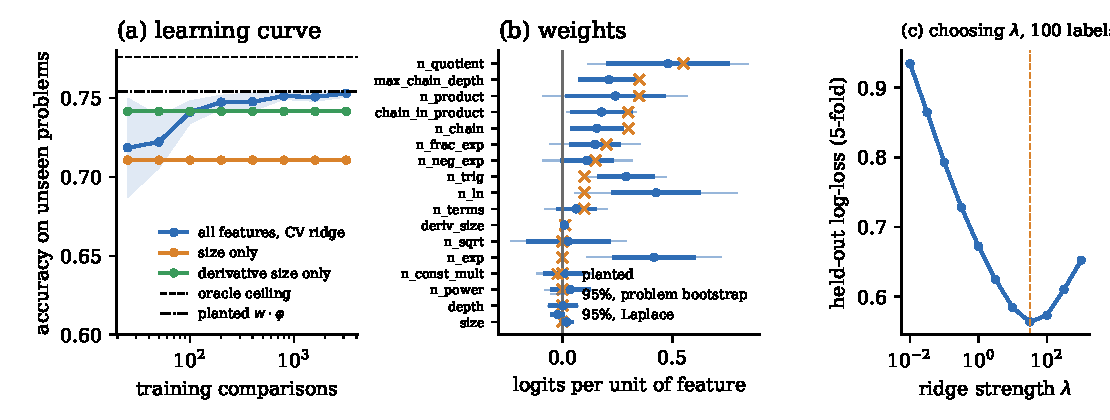
\includegraphics[width=\linewidth]{step06_feature_bt.pdf}
\caption{(a) Accuracy on unseen problems vs.\ number of training comparisons. (b) Learned vs.\ planted weights. (c) Five-fold
cross-validated log-loss against $\lambda$ with 100 training comparisons.}\label{fig:step06}
\end{figure}

\paragraph{Choosing $\lambda$ by cross-validation, and a bug.}
$\lambda$ is a \emph{hyperparameter}: it is not learned by minimizing the training loss (which always prefers $\lambda=0$). It is
chosen by estimating the held-out loss. \code{cv\_l2} splits the \emph{problems} into 5 folds. For each fold it trains on comparisons
among the other folds' problems and scores the comparisons that touch the held-out fold:

\codefrom{src/calcdiff/models/feature\_bt.py}
\begin{lstlisting}
for held in chunks:                          # chunks = 5 disjoint sets of problems
    te = pairs_touching(pairs, held)         # >= 1 held-out problem
    tr = ~te                                 # both problems in the other folds
    if te.sum() == 0 or tr.sum() == 0:
        continue
    for g, l2 in enumerate(grid):
        m = FeatureBT(l2=l2).fit(Phi, pairs[tr], y[tr])
        total[g] += te.sum() * log_loss(m.score(Phi), pairs[te], y[te])
    count += te.sum()
\end{lstlisting}
The first version required \emph{both} problems of a test comparison to be held out. With 25 comparisons spread over 350
problems, a fold of 70 problems then contained about $25\cdot(1/5)^2=1$ test comparison, sometimes zero. The mean of an empty
array is \code{nan}, and \code{np.argmin} returns the index of the \emph{first} \code{nan}. So CV silently ``chose'' the smallest $\lambda$
every time, and accuracy with 25 labels looked like $0.615$. With the fix it is $\GAccSmall$. Why is one held-out problem enough? A
feature model has no per-problem parameters, so a comparison between a seen problem and an unseen one still requires
\emph{scoring an unseen problem from its features}. (For item-level BT this would not be true.)

Panel (c) is the classic U-shaped curve: too little $\lambda$ overfits, too much underfits. The median chosen $\lambda$ rises from
$\GLamSmall$ at $m=25$ to $\GLamLarge$ at $m=3200$, which looks backwards until you notice that the loss is a \emph{sum} over comparisons.
The data term grows like $m$ while the penalty does not, so the effective strength is $\lambda/m$, which \emph{falls} from $\GLamRatioSmall$ to $\GLamRatioLarge$.
In Bayesian terms the prior $\theta\sim N(0,\lambda^{-1}I)$ is fixed, and it matters less as data accumulate.

\paragraph{Exercises.}
\begin{exercise}
Show that minimizing $\frac1m\sum_k\ell_k+\frac{\lambda'}2\|\theta\|^2$ is equivalent to our objective with $\lambda=m\lambda'$. Which
parametrization would you expect CV to make roughly constant in $m$, and why?
\end{exercise}
\begin{exercise}
Let $H$ be the Hessian at $\hat\theta$. Show the Laplace predictive variance of $\hat\delta(x)-\hat\delta(x')$ is
$(z-z')^\top H^{-1}(z-z')$. Why does it not depend on whether $x$ or $x'$ appeared in training?
\end{exercise}
\begin{exercise}
Explain precisely why ``touching'' test comparisons are a valid generalization test for the feature model but not for
item-level BT. Is the standardizer a (small) exception? (Look at which problems \code{fit} uses for $\mu,s$.)
\end{exercise}

%=============================================================================
\section{Collecting real labels}
\label{sec:labels}
%=============================================================================

Everything so far used a simulated instructor. This section builds the tool for the real one, and the theory for interpreting what it
collects. Run it with
\begin{center}
\verb|.venv/Scripts/python -m streamlit run labeler/app.py|
\end{center}
and open \url{http://localhost:8501}. It shows two problems side by side. You click \emph{Left is harder}, \emph{About the same},
or \emph{Right is harder}, and a new pair appears. A sidebar shows your count and your self-agreement on repeats, and has
an \emph{Undo} button. Under each problem there is a \emph{Flag as unnatural} button that removes the problem from rotation.

\paragraph{What is recorded, and why.}
Every click is one row in \file{data/labels.sqlite}:

\codefrom{src/calcdiff/labels/store.py}
\begin{lstlisting}
CREATE TABLE judgments (
    id          INTEGER PRIMARY KEY AUTOINCREMENT,
    left_id     TEXT NOT NULL REFERENCES problems(id),
    right_id    TEXT NOT NULL REFERENCES problems(id),
    outcome     TEXT NOT NULL CHECK (outcome IN ('left', 'right', 'tie')),
    labeler     TEXT NOT NULL,
    response_ms INTEGER,       -- time from showing the pair to the click
    is_repeat   INTEGER NOT NULL DEFAULT 0,
    created_at  REAL NOT NULL
);
\end{lstlisting}
Each column is there for a statistical reason:
\begin{itemize}[nosep]
\item \textbf{Screen position} (\code{left\_id}, \code{right\_id}, and the outcome \emph{relative to the screen}). People prefer one side more
  often than chance. With position recorded, we can fit $\P(\text{left}\succ\text{right})=\sigma(\delta_L-\delta_R+\beta)$. In design-matrix terms,
  $\beta$ is an \emph{intercept}, a column of ones in $D$. Section 6 said an intercept cancels in differences. That is true for
  difficulty, but not for a bias tied to the \emph{order} of presentation. Randomizing which problem goes left makes $\beta$
  statistically separable from $\delta$.
\item \textbf{Repeats} (\code{is\_repeat}). About 10\% of pairs are earlier pairs shown again with the sides swapped (so you can't
  just remember a position). They measure your own noise (below).
\item \textbf{Response time}. Slow judgments are plausibly close calls. We may later use it as a soft signal of $|\delta_i-\delta_j|$.
\item \textbf{Flags} (a separate table). These are data about the \emph{generator} rather than about difficulty: they show which corners of the grammar
  (Section 1) produce problems nobody would assign.
\end{itemize}

\paragraph{From clicks to training labels, including ties.}
\code{to\_arrays} turns rows into exactly what the models of Sections 4 and 6 consume: pairs $(L,R)$ and $y=1,0,\frac12$ for
left/right/tie. A tie with $y=\frac12$ contributes $\log(1+e^{t})-\frac t2$ to the cross-entropy, which is exactly half a win plus half a loss
(a test checks this). That is the simplest principled treatment. Davidson's model adds a separate tie parameter $\nu$,
$\P(\text{tie})\propto\nu\sqrt{\pi_i\pi_j}$, which we can try if you use the middle button a lot.

\paragraph{The scheduler.}

\codefrom{src/calcdiff/labels/schedule.py}
\begin{lstlisting}
def next_pair(store, labeler, rng):
    flagged = store.flagged()
    ids = [p.id for p in store.problems() if p.id not in flagged]
    past = [j for j in store.judgments(labeler) if not j.is_repeat and ...]
    if len(past) >= MIN_BEFORE_REPEATS and rng.random() < P_REPEAT:
        j = past[rng.integers(len(past))]
        return Pair(j.right_id, j.left_id, True)    # same pair, sides swapped
    i, k = rng.choice(len(ids), size=2, replace=False)
    return Pair(ids[i], ids[k], False)
\end{lstlisting}
For now pairs are uniformly random among the 300 pool problems. Section 4 told us this wastes effort: lopsided pairs have
conductance $\sigma'(\Delta)\approx0$. Section 10 replaces the last two lines with active learning, which picks the pair whose answer
would teach the model the most.

\paragraph{How the app works (Streamlit in one paragraph).}
Streamlit re-executes \file{labeler/app.py} from top to bottom on \emph{every} interaction. State that must survive a rerun lives in
\code{st.session\_state} (per browser tab: the current pair and the time it was shown) or in the database (permanent). The database
connection is created once per server process by a function decorated with \code{@st.cache\_resource}. On the very first launch, that
function also generates the pool of 300 problems (\code{Sampler(seed=2027)}). Buttons call functions \emph{before} the rerun via \code{on\_click}:

\codefrom{labeler/app.py}
\begin{lstlisting}
def submit(outcome: str) -> None:
    ms = int(1000 * (time.time() - state.shown_at))
    store.record(pair.left_id, pair.right_id, outcome, labeler, ms, pair.is_repeat)
    new_pair()                                   # choose the next pair; the rerun shows it

b1.button("Left is harder", on_click=submit, args=("left",), type="primary")
\end{lstlisting}

\paragraph{Thurstone or Bradley--Terry?}
Why the logistic link? Thurstone (1927) modeled a judgment as comparing \emph{noisy perceptions} $\delta_i+\varepsilon_i$ and
$\delta_j+\varepsilon_j$. With Gaussian $\varepsilon$ this gives $\P(i\succ j)=\Phi\bigl((\delta_i-\delta_j)/\sigma\sqrt2\bigr)$, the \emph{probit} model.
With i.i.d.\ \emph{Gumbel} $\varepsilon$, the difference is logistic, and we get exactly Bradley--Terry (Exercise~\ref{ex:gumbel}). Which noise
is right? The data can barely tell: $\Phi(t/\HProbitScale)$ differs from $\sigma(t)$ by at most $\HProbitGap$ anywhere
(Figure~\ref{fig:step07}(a)). We choose the logistic for convenience: closed-form gradients, and the same mathematics as logistic regression.

\paragraph{Reading your own consistency.}
Suppose that on a pair with gap $\Delta$ you pick the harder problem with probability $p=\sigma(|\Delta|)$, independently each time
it is shown. Then on a repeated pair you agree with yourself with probability $p^2+(1-p)^2$, while the best any model can do on
that pair is $p$. Averaging over pairs gives a curve linking two quantities: your overall self-agreement $A$, which the app measures,
and the ceiling $C$ on accuracy against your labels (Figure~\ref{fig:step07}(b)). For example, self-agreement of $70\%$, $80\%$ or $90\%$
means no model can exceed about $\HCeilAtSeventy$, $\HCeilAtEighty$ or $\HCeilAtNinety$ accuracy on your labels. This is the number to compare our models
against once real labels arrive: a model at $0.80$ is excellent if your ceiling is $0.82$, and mediocre if it is $0.93$.

\begin{figure}[h]\centering
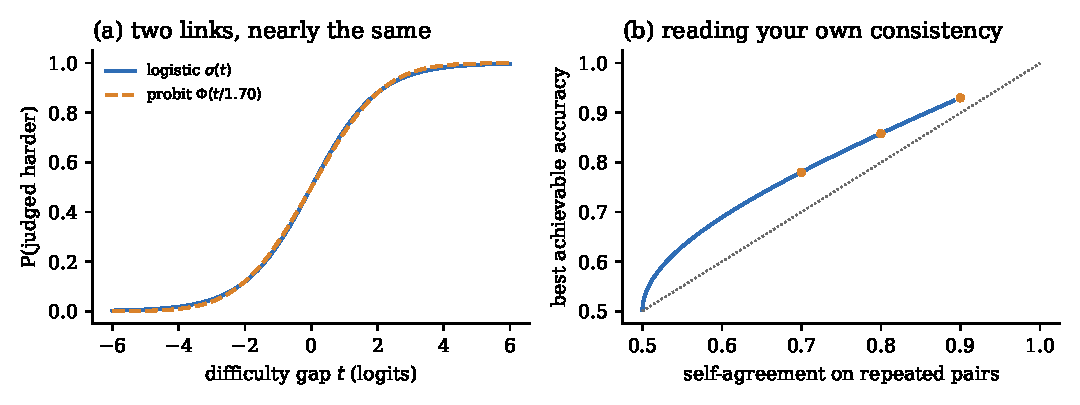
\includegraphics[width=0.92\linewidth]{step07_noise.pdf}
\caption{(a) Logistic and rescaled probit links. (b) Self-agreement on repeated pairs vs.\ the best accuracy achievable
against those labels, under the model of the last paragraph. Dots mark $70\%$, $80\%$, $90\%$ agreement.}\label{fig:step07}
\end{figure}

\paragraph{A labeling protocol.}
Some suggestions for when you sit down to label:
\begin{itemize}[nosep]
\item Decide what ``harder'' means, write it down, and stick to it. The app's prompt is ``for a typical Calculus I student, the work
  to find and write down the derivative''.
\item Go fast. Your first instinct is the measurement, and agonizing adds noise, not signal. Use \emph{About the same} when it really is.
\item Flag freely. A flagged problem costs nothing, while a weird problem in the training data costs accuracy.
\item 150 comparisons (about 20 minutes) is enough for a first model (Section 8). Section 6 says the feature model is
  near its ceiling at roughly one comparison per problem.
\end{itemize}

\paragraph{Exercises.}
\begin{exercise}\label{ex:gumbel}
Let $\varepsilon_i,\varepsilon_j$ be i.i.d.\ standard Gumbel, with $\P(\varepsilon\le u)=e^{-e^{-u}}$. Show that $\varepsilon_i-\varepsilon_j$ is standard logistic, so
that $\P(\delta_i+\varepsilon_i>\delta_j+\varepsilon_j)=\sigma(\delta_i-\delta_j)$.
\end{exercise}
\begin{exercise}
Writing the per-pair agreement as $a=p^2+(1-p)^2$ with $p\ge\frac12$, show $p=\frac12\bigl(1+\sqrt{2a-1}\bigr)$, and use Jensen's inequality
to prove the distribution-free bound $C\le\frac12\bigl(1+\sqrt{2A-1}\bigr)$. How close is the curve in Figure~\ref{fig:step07}(b) to this bound?
\end{exercise}
\begin{exercise}
With position randomized uniformly, show that the MLE of $\beta$ in $\sigma(\delta_L-\delta_R+\beta)$ is asymptotically uncorrelated with
the $\delta$'s. What goes wrong if the harder problem is shown on the left more often?
\end{exercise}

%=============================================================================
\section{Real labels: what the model learned about you}
\label{sec:real}
%=============================================================================

Everything up to now was rehearsal on a simulated instructor. This section fits the same code to $\RNJudg$ judgments you made in
the labeling app, and asks the questions Section 5 prepared: how good is the model, compared with what, and how sure are we?

\paragraph{The data.}
The $\RNJudg$ judgments include $\RNRepeats$ repeats and $\RNTies$ ties ($\RTiePct\%$) and cover $\RNProblemsSeen$ of the $\RNPool$ pool problems, about two
comparisons per problem. The median time per judgment was $\RMedianRT$\,s. Among decided comparisons you chose the left problem $\RLeftRate$ of
the time, so there is no detectable position bias (Section 7), and the intercept $\beta$ is not worth fitting. You flagged $\RNFlags$ problems.
The code path from the database to the model is the one from Section 7: \code{store.to\_arrays("dylan")} gives
\code{(problems, pairs, y)}, and \code{feature\_matrix} gives $\Phi$. Every number in this section is recomputed from the live database
whenever the notes are rebuilt, so it reflects the judgments as of the last build.

\paragraph{Your ceiling, and a subtlety about ties.}
You agreed with yourself on $\RAgreeAll$ repeats. Read naively through Figure~\ref{fig:step07}(b), that gives a ceiling around $0.87$, and
yet the models below score $\RAccFull$ and $\RAccDeriv$. Something had to give. Of your $\RDisagreeTotal$ disagreements, $\RDisagreeTie$ involve a \emph{tie} ("about the same" one time,
a decision the other). Accuracy skips tied labels, so the right comparison is agreement when \emph{both} showings were decided: $\RAgreeDD$. With so few
repeats the uncertainty is large. The Jeffreys interval (the posterior quantiles under a $\mathrm{Beta}(\frac12,\frac12)$ prior, which has good frequentist coverage
for small counts) is $[\RAgreeDDLo,\RAgreeDDHi]$, which maps to a ceiling of $\RCeilDD$ with range $[\RCeilDDLo,\RCeilDDHi]$. So the models are
\emph{at} your ceiling, as far as 22 repeats can tell. More repeats would sharpen this, and they are cheap: they come up automatically.

\paragraph{Cross-validated comparison.}
Every number below is out-of-fold: 5-fold CV over \emph{problems}, repeated 5 times. Inside each training fold, $\lambda$ is chosen by a
second, inner CV (\emph{nested} CV), so the held-out problems never influence any choice.

\codefrom{src/calcdiff/evaluate.py}
\begin{lstlisting}
def cross_val_diffs(Phi, pairs, y, make_model, rng, folds=5):
    ...
    for held in chunks:                          # disjoint sets of problems
        te = pairs_touching(pairs, held)
        model = make_model(pairs[~te], y[~te])   # never sees `held`; may run its own CV
        s = model.score(Phi)
        total[te] += s[pairs[te, 0]] - s[pairs[te, 1]]
        count[te] += 1
    return total / count                         # a comparison spanning 2 folds: average
\end{lstlisting}
Passing a \emph{factory} \code{make\_model} rather than a model is what makes nesting easy: the factory for the full model calls
\code{cv\_l2} on whatever training comparisons it is handed.

\begin{table}[h]\centering\small
\begin{tabular}{lcc}
\toprule
model & accuracy & log-loss \\
\midrule
constant (coin flip) & 0.500 & 0.693 \\
\code{size} only & 0.861 & 0.434 \\
\code{n\_chain} only & 0.850 & 0.403 \\
\code{depth} only & 0.870 & 0.394 \\
\code{deriv\_size} only & 0.925 & 0.378 \\
all 17 features, CV ridge & 0.914 & 0.310 \\
\bottomrule
\end{tabular}

\caption{Out-of-fold accuracy and log-loss on your labels. Single-feature models are one-parameter Bradley--Terry fits.}\label{tab:real}
\end{table}

Table~\ref{tab:real} has two surprises.
\begin{itemize}[nosep]
\item \textbf{One feature does almost everything.} \code{deriv\_size} alone orders $\RAccDeriv$ of your decided comparisons correctly
  (problem-bootstrap 95\% interval $[\RAccDerivLo,\RAccDerivHi]$). The full model gets $\RAccFull$, with interval $[\RAccFullLo,\RAccFullHi]$.
  As a working hypothesis about how you judge, \emph{harder means more to write down} is very good.
\item \textbf{Accuracy and log-loss disagree.} By log-loss the full model is better: $\RLLFull$ vs.\ $\RLLDeriv$. Is that real? Comparing the two
  separate intervals is the wrong test: they overlap, but the two models are scored on the \emph{same} comparisons, so their errors are correlated. A \emph{paired}
  bootstrap resamples problems once and recomputes \emph{both} losses on that resample. For the difference (full minus single-feature) it gives
  $[\RLLDiffLo,\RLLDiffHi]$. Nearly all of the mass is below zero, with the upper end at about zero, so the advantage is likely but not yet certain.
  (With 319 judgments the interval sat just below zero. Eleven more nudged it to the boundary, a reminder of how soft a ``significant'' result near the edge is.)
  Accuracy only checks the sign of $\hat\delta_i-\hat\delta_j$, while log-loss also checks its size.
  The full model knows \emph{how much} harder one problem is than another: when it is confident it is nearly always right, and when it is unsure it says so.
  That calibration matters downstream: comparing raters (Section 13) and an adaptive test (Section 14) both use the probabilities, not just the order.
\end{itemize}

\paragraph{Learning curves and the bias--variance trade-off.}
Why does the 1-feature model win on accuracy while the 17-feature model wins on log-loss? Fitting $d$ parameters to $m$ comparisons has a
predictable cost. For a correctly specified model fit by maximum likelihood, a second-order Taylor expansion around the true $\theta^\ast$
(Exercise~\ref{ex:aic}) gives
\[
  \E[\text{held-out loss}]-\E[\text{training loss}]\;\approx\;\frac{d}{m}\qquad\text{(Akaike, 1973)}.
\]
The training loss underestimates the truth by $\frac{d}{2m}$, because $\hat\theta$ was fit to these very points. The held-out loss overestimates it by
another $\frac{d}{2m}$, because $\hat\theta\ne\theta^\ast$. With a ridge penalty, $d$ is replaced by the \emph{effective degrees of freedom}
\[
  \mathrm{df}(\lambda)=\operatorname{tr}\bigl(H_{\text{data}}(H_{\text{data}}+\lambda I)^{-1}\bigr)=\sum_i\frac{\mu_i}{\mu_i+\lambda},
\]
where $\mu_i$ are the eigenvalues of the data Hessian. Each eigen-direction counts fully if the data dominate it ($\mu_i\gg\lambda$) and
not at all if the prior does. That's the Section 3 picture again: collinear directions have small $\mu_i$, and ridge switches them off.
\codefrom{scripts/figs\_step08.py}
\begin{lstlisting}
_, H_data = grad_hess(mdl.theta_, D, y[sub], 0.0)          # Hessian of the data term only
df = np.trace(H_data @ np.linalg.inv(H_data + mdl.l2 * np.eye(len(H_data))))
\end{lstlisting}
Figure~\ref{fig:step08}(a) holds out a fold of problems and trains on $m$ random comparisons from the rest (20 repetitions per $m$). The full model's
dotted line, training loss $+\,\mathrm{df}/m$, tracks its held-out loss: predicted gap $\RGapPredTwentyFive$ vs.\ observed $\RGapObsTwentyFive$ at $m=25$,
and $\RGapPredTwoHundred$ vs.\ $\RGapObsTwoHundred$ at $m=200$ (where $\mathrm{df}\approx\RDFAtTwoHundred$ of 17). The prediction runs high at small $m$,
which is plausible: $\lambda$ is re-tuned at each $m$, the theory assumes a fixed model, and it is an $m\to\infty$ expansion. The $1/m$ shape is right. This is the bias--variance trade-off in its
cleanest form:
\begin{itemize}[nosep]
\item \code{deriv\_size} only: $\mathrm{df}=1$, so almost no variance. But it plateaus at the log-loss of the best \emph{one-feature} model.
  That plateau is its \emph{bias}.
\item All features: more variance (a $\mathrm{df}/m$ penalty), less bias. With 25 comparisons it already beats the simple model on log-loss
  ($\RLLFullTwentyFive$ vs.\ $\RLLDerivTwentyFive$), but not on accuracy ($\RAccFullTwentyFive$ vs.\ $\RAccDerivTwentyFive$).
\end{itemize}

\begin{figure}[h]\centering
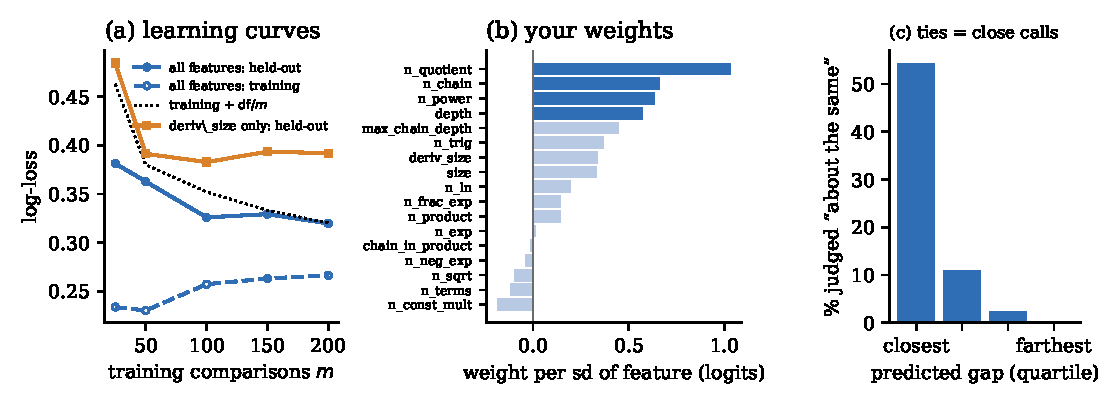
\includegraphics[width=\linewidth]{step08_real.pdf}
\caption{Your labels. (a) Training and held-out log-loss vs.\ training-set size, and the Akaike/TIC prediction.
(b) Standardized weights of the final model (dark: problem-bootstrap $|z|>1.96$). (c) Fraction of ``about the same'' answers by quartile of the model's predicted gap.}\label{fig:step08}
\end{figure}

\paragraph{What the weights say about you.}
Fit on all comparisons (CV chooses $\lambda=\RLamAll$), the final model's scores have Spearman correlation $\RRhoScoreDeriv$ with derivative size.
Intervals here come from the problem bootstrap of Section 6, not from Laplace. (On your labels the two happen to agree, with a median ratio of $\RRealSERatio$.
That suggests the features leave little problem-specific residual in your judgments, unlike the simulated instructor, whose $\tau\varepsilon$ the features could not see.)
Only $\RNSig$ weights have bootstrap $|z|>1.96$. That is the collinearity of Section 3 at work: the data can't split credit among
\code{size}, \code{depth}, the rule counts and \code{deriv\_size}, which all move together. Panel (b) shows the standardized weights. The largest are on
$\RTopStd$.

One effect stands clear of the rest, and it shows how to read a weight carefully. \textbf{A quotient rule adds $\RQuotW$ logits} beyond everything else
the model sees: bootstrap 95\% interval $[\RQuotLo,\RQuotHi]$, positive in $\RQuotFracPos\%$ of 500 resamples. The \emph{direction} is solid. You treat
quotients as harder than their size alone explains, which is a genuinely pedagogical finding, and the kind of thing to check on a second instructor.
The \emph{size} is not solid. Only $\RFracQuot\%$ of the problems you saw contain a quotient, so the estimate leans on few comparisons and on the prior. It is
$\RQuotSmallLam$ logits at $\lambda=0.316$ and $\RQuotLargeLam$ at $\lambda=31.6$, against $\RQuotW$ at the CV choice. A weight that moves this much with the
regularization should be reported as a direction with a wide range, not as ``a quotient multiplies the odds by $e^{\RQuotW}$''.

\paragraph{Do ties mean ``close''? A check on the model itself.}
Bradley--Terry never saw a tie as anything but half a win. If the model is a good description of your judgments, your ties should
concentrate where its \emph{out-of-fold} predicted gap $|\hat\delta_i-\hat\delta_j|$ is small. Figure~\ref{fig:step08}(c) shows exactly that: $\RTieLowGap\%$ ties in the
closest quartile and $\RTieHighGap\%$ in the farthest. Your response times agree: a median of $\RRTLowGap$\,s on the closest pairs vs.\ $\RRTHighGap$\,s on the most
lopsided. A model that predicts things it was never trained on (ties, hesitation) is a model worth trusting.

\paragraph{Error analysis.}
The model gets $\RNWrong$ decided comparisons wrong out-of-fold. Table~\ref{tab:errors} lists the five it was most confident about. Reading
your own disagreements with a model is the most useful thing in this section. Some are probably slips: with a $\RMedianRT$-second median, a few misclicks are
inevitable, and the most confident miss is a candidate. Others are real disagreements about what makes a problem hard. For instance, you rated
$8\sin(\ln(x^2)+7)$ harder than $\cos(\cos(e^{x^3}-5))$, while the model, which counts nested compositions, disagreed. Where you think \emph{you} are right,
the remedy is a feature, not more data.

\begin{table}[h]\centering\footnotesize
{\renewcommand{\arraystretch}{1.7}\begin{tabular}{llc}
\toprule
you said harder & model said harder & $P_{\text{model}}$ \\
\midrule
$\displaystyle x^{2} + \left(\left(x^{1/3} + 3\right)^{4} - 3\right)^{2}$ & $\displaystyle x^{3} + 7 \left(-4 x^{1/2}\right) \sin\left(x^{-1} e^{-5 x^{2} + 1}\right)$ & 0.98 \\
$\displaystyle x^{4} + x^{3} + \sqrt{\sin\left(x^{3}\right) + 5} + 4$ & $\displaystyle x^{-1} + x^{1/2} + \frac{\sqrt{4 x^{3}}}{2 x^{3/2}} + 2$ & 0.94 \\
$\displaystyle x^{-1/2} e^{x^{4}} + 4$ & $\displaystyle \ln x + \sqrt{x} + e^{-7 x^{3}} \cos\left(x^{3/2} - 8\right)$ & 0.91 \\
$\displaystyle 8 \sin\left(\ln\left(x^{2}\right) + 7\right)$ & $\displaystyle \cos\left(\cos\left(e^{x^{3}} - 5\right)\right)$ & 0.84 \\
$\displaystyle \frac{e^{x^{3/2}}}{\left(x^{2} - 3\right)^{2}} + 4 x + 2 \left(7 x^{3} + 1\right)^{5}$ & $\displaystyle -2 x^{2} + 2 \left(\sqrt{e^{x^{2} + 2}} - 6\right)^{4} \cdot 9 x \sin\left(x^{-2}\right) x$ & 0.81 \\
\bottomrule
\end{tabular}}

\caption{The model's five most confident out-of-fold mistakes. $P_{\text{model}}$ is the probability it gave to the answer you did not choose.}\label{tab:errors}
\end{table}

The table also caught a bug in Section 1's generator. Terms like $3\cdot 9x(\ldots)$ and $7(-4x^{1/2})\sin(\ldots)$ stack two coefficients, which
\code{is\_natural} should have rejected and no instructor would write. (You didn't flag them, perhaps because they read as merely ugly rather than
wrong.) The fix is in Section 1. Under the tightened rule, $\RNAutoFlags$ of the $\RNPool$ pool problems are unnatural, and $\RNDropped$ of your judgments involve one.
What to do with data collected under a bug? Here the judgments are still honest comparisons of real expressions, so they stay in the training set.
The $\RNAutoFlags$ problems are flagged under a separate labeler name, \code{auto:is\_natural}, which takes them out of rotation without being mistaken for your own flags.
Then a \emph{robustness check}: refit without the $\RNDropped$ judgments. Accuracy is $\RAccKeep$ and log-loss $\RLLKeep$ (vs.\ $\RAccFull$ and $\RLLFull$), and the
quotient weight is $\RQuotKeep$ with interval $[\RQuotKeepLo,\RQuotKeepHi]$. The conclusions do not hinge on the bad problems. Data inspection found this
bug, not a test, and that is typical.

\paragraph{Exercises.}
\begin{exercise}\label{ex:aic}
Let $\ell$ be a log-loss with $\theta^\ast=\arg\min\E\ell$, $J=\E\nabla^2\ell(\theta^\ast)$, $K=\Var\nabla\ell(\theta^\ast)$. Show that, to order $1/m$,
$\E[\text{held-out}]-\E[\text{train}]=\operatorname{tr}(J^{-1}K)/m$ (Takeuchi), and that $J=K$ for a correctly specified likelihood, giving $d/m$.
\end{exercise}
\begin{exercise}
Show that $\mathrm{df}(\lambda)=\sum_i\mu_i/(\mu_i+\lambda)$ is decreasing in $\lambda$, with $\mathrm{df}(0)=\operatorname{rank}H_{\text{data}}$. Interpret each term as the
fraction of the $i$-th eigen-direction that is ``learned from data'' rather than ``taken from the prior''.
\end{exercise}
\begin{exercise}
Construct three problems and probabilities for which a model $A$ orders every pair correctly but has worse expected log-loss than a
model $B$ that misorders one pair. What does this say about which metric to use for model \emph{selection} vs.\ \emph{reporting}?
\end{exercise}

%=============================================================================
\section{Gradient boosting: gradient descent in function space}
\label{sec:boosting}
%=============================================================================

The linear model can only add up feature effects: one more chain rule is worth the same everywhere. Section 3 handled
\emph{one} interaction by hand (\code{chain\_in\_product}) and noted that this does not scale. Gradient-boosted trees learn
nonlinearities and interactions automatically. They are the default winner on tabular data in practice, and the idea behind them is
a beautiful piece of optimization.

\paragraph{Descent on scores, projected onto trees.}
Forget parameters for a moment, and optimize the scores $F_i=\hat\delta(x_i)$ of the training problems directly. The loss
$L(F)=\sum_k[\log(1+e^{F_i-F_j})-y_k(F_i-F_j)]$ is the Bradley--Terry loss with one-hot design, so (Section 4) its gradient and Hessian are
\[
  g=\nabla_FL=D^\top(p-y),\qquad \nabla_F^2L=D^\top WD=L_w,\ \text{the weighted Laplacian.}
\]
Plain gradient descent on $F$ would just fit item-level BT. It moves each $F_i$ independently and says nothing about unseen problems. Boosting
instead \emph{restricts every step to a function of the features}. Each round fits a small regression tree $f_t:\R^d\to\R$ to the descent
direction, then steps $F\leftarrow F+\nu f_t(\varphi(x))$. After $T$ rounds, $\hat\delta(x)=\nu\sum_tf_t(\varphi(x))$ can score any problem. Friedman (2001) called this
\emph{gradient boosting}.

Which tree? Expand $L$ to second order along a step $f$, replacing $L_w$ by its diagonal $h_i=(L_w)_{ii}$:
\[
  L(F+f)\approx L(F)+\sum_ig_if_i+\tfrac12\sum_ih_if_i^2=\tfrac12\sum_ih_i\Bigl(f_i+\frac{g_i}{h_i}\Bigr)^2+\text{const}.
\]
So the best tree is a \emph{weighted least-squares} fit to the per-problem Newton steps $-g_i/h_i$, with weights $h_i$. That is a standard regression tree,
exactly what \code{DecisionTreeRegressor} fits.

\codefrom{src/calcdiff/models/boosted\_bt.py}
\begin{lstlisting}
def problem_grad_hess(F, pairs, y):
    p = expit(F[pairs[:, 0]] - F[pairs[:, 1]])
    r = p - y                      # d loss_k / d t_k: the "lambda" of LambdaRank
    w = p * (1 - p)                # d2 loss_k / d t_k^2
    g = np.bincount(pairs[:, 0], r, n) - np.bincount(pairs[:, 1], r, n)
    h = np.bincount(pairs[:, 0], w, n) + np.bincount(pairs[:, 1], w, n)
    return g, h, w
\end{lstlisting}
\code{np.bincount(idx, weights, n)} sums \code{weights} into bins \code{idx}: it is $D^\top r$ without forming $D$. (A test checks that $g$ and $h$ agree
with \code{grad\_hess} on the one-hot design.) The quantity $r_k=p_k-y_k$ is what the ranking literature calls the \emph{lambda} of a pair, and
\emph{LambdaMART}, the algorithm behind many search engines' rankers, is precisely this construction.

\paragraph{The leaf values: an exact Newton step, and a graph cut.}
The tree decides the \emph{partition}. We then choose each leaf's value by an exact one-dimensional Newton step instead of the
diagonal approximation. Shifting the scores of all problems in a leaf $R$ by $\gamma$ moves $F$ along $\mathbf 1_R$, so
\begin{align*}
  \frac{d}{d\gamma}L(F+\gamma\mathbf 1_R)&=\mathbf 1_R^\top g=\sum_{i\in R}g_i,\\
  \frac{d^2}{d\gamma^2}L(F+\gamma\mathbf 1_R)&=\mathbf 1_R^\top L_w\mathbf 1_R=\sum_kw_k\bigl(\mathbf 1_R(i_k)-\mathbf 1_R(j_k)\bigr)^2=\operatorname{cut}_w(R).
\end{align*}
The curvature in direction $\mathbf 1_R$ is the total weight of comparisons with exactly one problem in $R$. A comparison \emph{inside} the leaf is
unaffected by shifting both of its problems together. That is the Laplacian quadratic form from Section 4 again, now evaluated on an indicator vector,
where it becomes a graph cut. The diagonal approximation would use $\sum_{i\in R}h_i=\operatorname{cut}_w(R)+2w(\text{inside }R)$
(Exercise~\ref{ex:cut}), which overestimates the curvature and makes the steps too timid.

\codefrom{src/calcdiff/models/boosted\_bt.py}
\begin{lstlisting}
for _ in range(self.n_trees):
    g, h, w = problem_grad_hess(F, pairs, y)
    tree.fit(Phi[items], -g[items] / h[items], sample_weight=h[items])  # partition
    leaf_of = tree.apply(Phi)                                 # leaf id of EVERY problem
    G = np.bincount(leaf_of[items], g[items], n_nodes)        # sum of g per leaf
    value = -G / (leaf_cut(leaf_of, pairs, w, n_nodes) + self.leaf_l2)  # Newton
    F += self.learning_rate * value[leaf_of]                  # shrunken step

def leaf_cut(leaf_of, pairs, w, n_leaves):
    li, lj = leaf_of[pairs[:, 0]], leaf_of[pairs[:, 1]]
    cross = li != lj                                          # comparisons crossing a leaf
    return (np.bincount(li[cross], w[cross], n_leaves)
            + np.bincount(lj[cross], w[cross], n_leaves))
\end{lstlisting}
Two tests pin the mathematics down. \code{test\_leaf\_curvature\_is\_the\_laplacian\_cut} checks
$\operatorname{cut}_w(R)=\mathbf 1_R^\top L_w\mathbf 1_R$ against the explicit Hessian, and \code{test\_leaf\_value\_is\_exact\_newton\_step\_for\_one\_leaf}
checks $\gamma$ against finite differences. \code{leaf\_l2} adds a ridge penalty $\frac{\lambda}{2}\gamma^2$ to each leaf (the XGBoost convention).

\paragraph{What trees can express, and what they ignore.}
A tree of depth $D$ is a piecewise-constant function on axis-aligned boxes, and each leaf is reached by at most $D$ comparisons $\varphi_j\le c$. Hence:
\begin{itemize}[nosep]
\item \textbf{Depth controls the order of interactions.} A depth-1 tree (a ``stump'') splits on one feature, so a sum of stumps is an
  \emph{additive} model $\sum_jf_j(\varphi_j)$: nonlinear in each feature, but with no interactions. Depth $D$ allows interactions among up to $D$ features.
\item \textbf{Invariance to monotone transformations.} Replacing $\varphi_j$ by any strictly increasing $u(\varphi_j)$ yields the same partitions,
  hence the same model (\code{test\_invariant\_to\_monotone\_feature\_transforms}). No standardization is needed. Contrast this with ridge (Section 3).
\item \textbf{Regularization} comes from four knobs: the shrinkage $\nu$, the depth, the minimum leaf size, and above all the \emph{number of trees}, chosen by
  early stopping. \code{cv\_n\_trees} fits once per fold and reads off the held-out loss after every tree, so the whole curve costs a single fit.
\end{itemize}

\paragraph{Inductive bias decides the winner.}
Figure~\ref{fig:step09}(a,b) compares linear BT with boosted trees (depth 2) on two synthetic truths, using held-out log-loss.
\begin{itemize}[nosep]
\item \textbf{Linear truth} (the simulated instructor of Section 4): linear wins, by a lot at small $m$ ($\QLinTruthLinSmall$ vs.\ $\QLinTruthBoostSmall$ with 100 comparisons)
  and still at $m=3200$ ($\QLinTruthLinLarge$ vs.\ $\QLinTruthBoostLarge$). Trees approximate a linear function with a staircase, which wastes data.
\item \textbf{Interaction truth}: chain rules make a problem \emph{harder} when a quotient is present and \emph{easier} without one. No linear model can express that.
  Boosting overtakes linear from $m=\QIntCross$ and approaches the oracle ($\QIntTruthBoostLarge$ vs.\ $\QIntTruthOracle$, linear $\QIntTruthLinLarge$).
\end{itemize}
Neither model is ``better''. Each encodes a bet about the truth, and data decide which bet pays (the \emph{no-free-lunch} theorem made concrete).
Note the sizes of the gaps, too. Even a sign-flipping interaction shows up only modestly in the averages, because quotients are rare. Interactions that touch
few problems are hard to detect, for any method.

\paragraph{On your labels.}
Out-of-fold over $\QNJudg$ judgments (5-fold CV over problems, repeated 5 times; the number of trees is chosen by inner CV), boosting scores accuracy
$\QRealAccBoost$ and log-loss $\QRealLLBoost$, against $\QRealAccLin$ and $\QRealLLLin$ for linear BT. The paired problem-bootstrap interval for the log-loss difference
(boosted minus linear) is $[\QRealDiffLo,\QRealDiffHi]$, which straddles zero. \emph{At this sample size the two are indistinguishable.} That itself is information:
whatever structure trees could add, 330 comparisons do not reveal it.

Figure~\ref{fig:step09}(c) asks the sharper question of which tree depth is best. Held-out log-loss bottoms out at $\QBestLLDepthOne$ for depth 1 (after $\QBestTreesDepthOne$ trees),
$\QBestLLDepthTwo$ for depth 2, and $\QBestLLDepthFour$ for depth 4. Then every curve turns upward as the trees start fitting noise. Depth 4 ends at
$\QFinalLLDepthFour$ held-out while its training loss falls to $\QFinalTrainDepthFour$, the textbook signature of overfitting. \textbf{The best model is a sum of stumps:
an additive model with no interactions.} So there is no evidence of interactions in how you judge difficulty, at least none these features can express. Whatever
boosting gains over linear BT comes from bending individual features, not from combining them. The boosted model leans mostly on $\QGainTop$ (share of total
split gain). As in Section 8, that is ``how much there is to write'' doing most of the work.

A caution about gain: it credits whichever of several correlated features a tree happened to split on, so it is not a reliable account of
\emph{why} the model predicts what it does. Section 12 replaces it with Shapley values, which have axioms behind them.

\begin{figure}[h]\centering
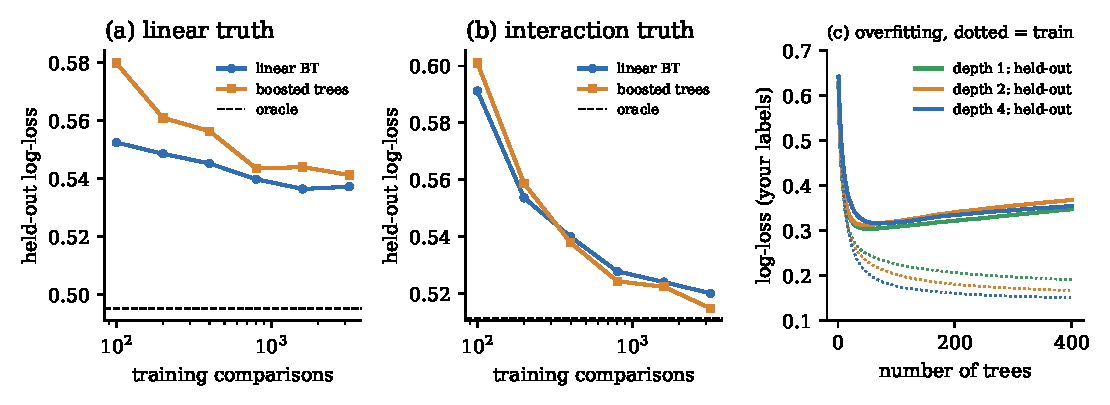
\includegraphics[width=\linewidth]{step09_boosting.pdf}
\caption{(a,b) Held-out log-loss of linear and boosted Bradley--Terry on synthetic truths, against training-set size. (c) Your labels:
held-out (solid) and training (dotted) log-loss against the number of trees for depths 1, 2 and 4.}\label{fig:step09}
\end{figure}

\paragraph{Exercises.}
\begin{exercise}\label{ex:cut}
Show that $\sum_{i\in R}(L_w)_{ii}=\operatorname{cut}_w(R)+2\,w(E(R))$, where $E(R)$ is the set of comparisons with both problems in $R$. Conclude that the
diagonal Newton step $-\sum_{i\in R}g_i/\sum_{i\in R}h_i$ is never larger in magnitude than the exact one.
\end{exercise}
\begin{exercise}
Prove that boosting with depth-1 trees produces a function of the form $\sum_jf_j(\varphi_j)$ with each $f_j$ a step function, and that every such function on a
finite data set can be reached. Which simple feature-wise shape (monotone? convex?) would you impose on $f_{\code{deriv\_size}}$ as an instructor, and how
could you enforce it?
\end{exercise}
\begin{exercise}
Show that boosting with a learning rate $\nu\to0$ and $T\nu$ fixed traces a path that, for an \emph{additive} model class, resembles the ridge path in $\lambda$:
early stopping acts as regularization. (A heuristic argument suffices. Look up ``boosting as $\ell_1$-regularized path following'' for the precise
statement in the linear case.)
\end{exercise}

%=============================================================================
\section{Active learning: which question to ask next}
\label{sec:active}
%=============================================================================

Your time is the scarce resource. Section 4 showed that comparisons are not equally informative: a lopsided pair has
conductance $\sigma'(\Delta)\approx0$ and teaches almost nothing. So instead of showing random pairs, let the current model
choose. This section is a cautionary tale with a happy ending. The obvious choice rules made things \emph{worse}, and
finding out why led to a better model, not just a better rule.

\paragraph{Bayesian experimental design.}
After fitting, the model has an approximate posterior $\theta\sim N(\hat\theta,\Sigma)$, with $\Sigma=H^{-1}$ (Laplace, Section 4). A candidate pair with
feature difference $d=z_i-z_j$ has predicted probability $p=\sigma(\hat\theta\cdot d)$, and asking it would add $w\,dd^\top$ to the precision, with $w=p(1-p)$.
Notably, the update does not depend on the \emph{answer}, so we can evaluate it before asking. Two consequences follow from rank-one linear algebra:
\begin{itemize}[nosep]
\item \emph{Matrix determinant lemma}: $\det(H+w\,dd^\top)=\det H\,(1+w\,d^\top\Sigma d)$. The entropy of a Gaussian is $\frac12\log\det\Sigma+$const,
  so the expected information gain about $\theta$ is
  \[ \mathrm{EIG}=\tfrac12\log\bigl(1+w\,s^2\bigr),\qquad s^2=d^\top\Sigma d. \]
  Maximizing it greedily is sequential \emph{D-optimal} design (``D'' for determinant).
\item \emph{Sherman--Morrison}: $\Sigma'=\Sigma-c\,\Sigma dd^\top\Sigma$ with $c=w/(1+ws^2)$. If what we care about is predicting
  \emph{typical} pairs, i.e.\ the average predictive variance $\E_{d'}[d'^\top\Sigma d']=\operatorname{tr}(\Sigma C)$ with $C=\E[d'd'^\top]$ over random pairs, then the pair
  that reduces it most maximizes
  \[ c\;d^\top\Sigma C\Sigma d. \]
  That is \emph{V-optimal} design (``V'' for variance; Kiefer's alphabet has many more letters).
\end{itemize}
The simplest heuristic, \emph{uncertainty sampling}, uses $w$ alone: it asks the closest call. Both $w$ and $s^2$ matter. A close call ($w$
large) whose answer moves the model in a direction it is already sure about ($s^2$ small) is wasted.

\codefrom{src/calcdiff/active.py}
\begin{lstlisting}
Z = model.scaler_.transform(model._select(Phi))
D = Z[cand[:, 0]] - Z[cand[:, 1]]                 # one row d_k per candidate pair
p = expit(D @ model.theta_)
w = p * (1 - p)
if strategy == "uncertainty":
    return w
Sigma = model.fit_.covariance()
s2 = np.einsum("kj,jl,kl->k", D, Sigma, D)        # d_k^T Sigma d_k, all k at once
if strategy == "information":
    return 0.5 * np.log1p(w * s2)                  # D-optimal
if strategy == "variance":
    C = 2 * np.cov(Z[np.unique(cand)], rowvar=False)   # E[d d^T] for random pairs
    SD = D @ Sigma
    return w / (1 + w * s2) * np.einsum("kj,jl,kl->k", SD, C, SD)   # V-optimal
\end{lstlisting}
\code{np.einsum("kj,jl,kl->k", D, Sigma, D)} computes all $\approx$45{,}000 quadratic forms $d_k^\top\Sigma d_k$ in one vectorized call, with no Python loop.
(Why $C=2\operatorname{Cov}(z)$? If $z,z'$ are independent draws, $\E[(z-z')(z-z')^\top]=2\operatorname{Cov}(z)$.)
The test \code{test\_information\_gain\_is\_half\_log\_det\_ratio} checks the EIG formula against explicit log-determinants.
The function \code{choose} then takes the argmax, except with probability 10\% it picks uniformly at random (\emph{exploration}). A purely greedy
learner can lock onto whatever its current, possibly wrong, model finds interesting and never see evidence against it.

\paragraph{The simulation loop.}

\codefrom{src/calcdiff/active.py}
\begin{lstlisting}
def ask(k):                                        # each pair is answered exactly once
    chosen.append(k); labels.append(answer(k)); remaining[k] = False

for k in rng.choice(len(cand), size=n_start, replace=False):
    ask(int(k))                                    # a random start
while True:
    model = make_model().fit(Phi, cand[chosen], np.array(labels))
    ... evaluate(model) ...
    for _ in range(batch):                         # `batch` picks per refit
        left = np.flatnonzero(remaining)
        ask(int(left[choose(model, Phi, cand[left], strategy, rng, explore)]))
\end{lstlisting}
\code{answer(k)} is either a simulated instructor or a lookup of one of your stored judgments, so the same loop runs both experiments below. My first
version called \code{answer} again at every refit. For a simulated instructor that re-draws the coin and gives a pair a \emph{different} label each time. The
\code{ask} helper fixes this, and \code{test\_loop\_asks\_each\_pair\_once\_and\_never\_relabels} guards it.

\paragraph{First result: the obvious rules backfire.}
On the simulated instructor of Section 4 (a pool of 300 problems like the app's, held-out log-loss on 150 unseen problems, 8 seeds, refit every $\ABatch$ labels),
Figure~\ref{fig:step10}(a):
\begin{itemize}[nosep]
\item \textbf{Uncertainty sampling is harmful}, and it gets worse with more data: $\ALLUncHundred$ at 100 labels and $\ALLUncFinal$ at $\ANTotal$, against
  $\ALLRandHundred$ and $\ALLRandFinal$ for random. Its asked pairs have a mean true gap of only $\AGapUnc$ logits (random: $\AGapRand$). Near a gap of 0 the instructor's answer
  is a coin flip, so uncertainty sampling diligently collects coin flips, and only along directions the model has already pinned down.
\item \textbf{D-optimal design helps at first and then degrades}: $\ALLInfoSixty$ vs.\ $\ALLRandSixty$ at 60 labels, but $\ALLInfoFinal$ vs.\ $\ALLRandFinal$ at $\ANTotal$.
  Panel (b) shows why: one problem gets asked up to $\AMaxUseInfo$ times (random: $\AMaxUseRand$). The determinant is shrunk fastest by \emph{unusual} problems, the high-leverage
  points in feature space, so D-optimality keeps returning to the outliers.
\end{itemize}

\paragraph{Diagnosis: the acquisition function inherits the model's blind spot.}
Recall the planted truth $\delta(x)=w\cdot\varphi(x)+\tau\varepsilon(x)$. The part $\tau\varepsilon(x)$ belongs to the \emph{problem}, and every comparison involving $x$ shares it.
The feature model has no term for it. It believes each comparison is fresh, independent evidence about $\theta$, so it sees no harm in asking about the same
outlier a fifth time. In fact the fifth comparison mostly measures that problem's own $\varepsilon$, and fitting it pulls $\theta$ the wrong way. Two
quick experiments confirmed this. With $\tau=0$ (no per-problem quirks) D-optimal design matched or beat random. With $\tau=0.5$ it
got worse with more data. This is the third time the same fact has mattered (Sections 5, 6, 8): \emph{problems, not comparisons, are the independent units}.

\paragraph{The fix: put the blind spot into the model.}
Give every problem its own random effect,
\[
  \delta(x_i)=\theta\cdot z_i+u_i,\qquad u_i\overset{\text{iid}}\sim N(0,\tau^2),
\]
a \emph{mixed model} (fixed effects $\theta$, random effects $u$). The design row becomes $a=[\,z_i-z_j,\ e_i-e_j\,]$ and the prior on $u$ is a ridge penalty
$1/\tau^2$ on those coordinates, so the Section 4 fitter works unchanged once it accepts a per-coordinate penalty:

\codefrom{src/calcdiff/models/mixed\_bt.py}
\begin{lstlisting}
G = np.hstack([self.Z_, np.eye(n)])                # row i: g_i = [z_i, e_i]
D = G[pairs[:, 0]] - G[pairs[:, 1]]                # a = g_i - g_j
prior = np.concatenate([np.full(d, self.l2), np.full(n, 1.0 / self.tau ** 2)])
self.fit_ = fit_newton(D, y, l2=prior)             # ridge = Gaussian prior, per coordinate
\end{lstlisting}
Now the design criterion should measure information about $\theta$ \emph{alone}, since that is the part that generalizes to unseen problems. The joint
covariance gets a rank-one update, and its $\theta$-block becomes $\Sigma_{\theta\theta}-c\,vv^\top$ with $v=(\Sigma a)_\theta$. So, by the determinant lemma once more,
\[
  \mathrm{EIG}_\theta=-\tfrac12\log\bigl(1-c\,v^\top\Sigma_{\theta\theta}^{-1}v\bigr),\qquad
  \text{V-optimal: }\ c\,v^\top Cv .
\]
When a problem's $u_i$ is already pinned down, asking about it again still informs $\theta$. When it isn't, most of the answer goes into $u_i$, and the
formulas know that. Two tests check this: one against brute-force log-determinants of the inverted joint precision, and one showing that the mixed criterion reduces to the plain one as
$\tau\to0$.

\paragraph{Results.}
Combining the two ideas, V-optimal design (target the loss we are scored on) on the mixed model (respect the per-problem dependence), gives the
blue curve in Figure~\ref{fig:step10}(a):
$\ALLVarSixty$, $\ALLVarHundred$, $\ALLVarTwoHundred$ and $\ALLVarFinal$ at 60, 100, 200 and $\ANTotal$ labels, against random's $\ALLRandSixty$, $\ALLRandHundred$, $\ALLRandTwoHundred$, $\ALLRandFinal$.
It reaches random's 200-label loss with about $\AVarNeedsForTwoHundred$ labels, roughly $\ASavingTwoHundred\%$ fewer, while asking any one problem at most $\AMaxUseVar$ times.
Because every seed uses the same starting pairs and test set for every strategy, the honest test is the \emph{paired} difference across seeds. V-optimal minus random is
$\ADiffVarTwoHundred\pm\ADiffSEVarTwoHundred$ at 200 labels (lower in $\AWinsVarTwoHundred$ of $\ASeeds$ seeds) and $\ADiffVarThreeHundred\pm\ADiffSEVarThreeHundred$ at $\ANTotal$
(lower in $\AWinsVarThreeHundred$ of $\ASeeds$).
The direction is consistent, but the effect is under two standard errors: \emph{suggestive, not conclusive} at 8 seeds. The same paired test puts
D-optimal at $\ADiffInfoSixty\pm\ADiffSEInfoSixty$ at 60 labels but $\ADiffInfoTwoHundred\pm\ADiffSEInfoTwoHundred$ at 200, its early lead gone. The honest summary:
uncertainty sampling clearly hurts (by an order of magnitude more than any other difference here), D-optimal design is a gamble, and V-optimal + mixed is a
modest, steady improvement, worth roughly a fifth of the labels in the middle of the curve. Active learning is famous for large gains in settings with many
parameters and cheap candidate pools. With 17 parameters, random pairs are already a decent design, and the main lesson is \emph{not to make things worse}.

\paragraph{Replay on your labels.}
We can test on real data without new clicks. In each fold of the problem-level CV, the candidate set is the comparisons you already made among
training problems, and ``asking'' reveals your stored answer. Panel (c) shows the result. At 60 labels, V-optimal + mixed gives held-out log-loss $\AReplayVarSixty$ (D-optimal $\AReplayInfoSixty$)
against $\AReplayRandSixty$ for random, and it matches random's 100-label loss with $\AReplayVarReach$ labels. The effect is small but in the same direction. Replay understates
the benefit, because the strategies can only choose among pairs that random sampling happened to produce.

\begin{figure}[h]\centering
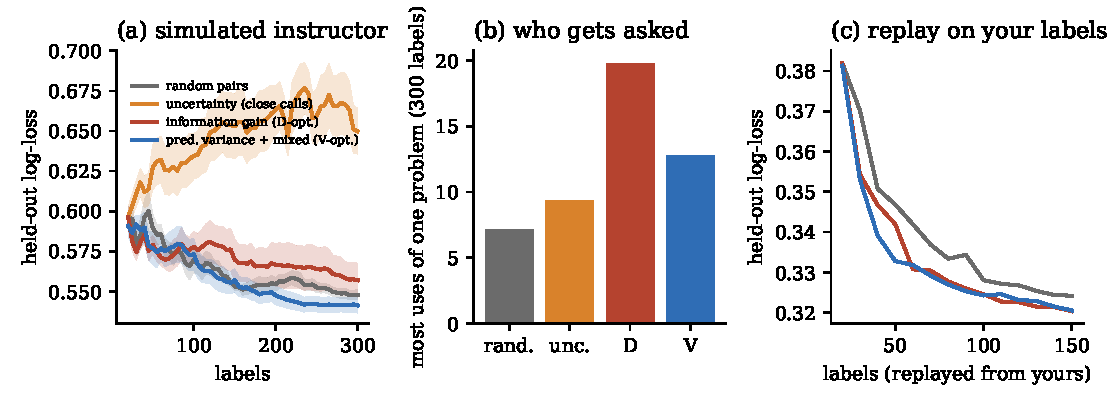
\includegraphics[width=\linewidth]{step10_active.pdf}
\caption{(a) Held-out log-loss vs.\ labels on the simulated instructor (mean $\pm$ s.e.\ over 8 seeds). (b) The most times any single problem
was asked. (c) Replay on your labels, choosing only among comparisons you already made.}\label{fig:step10}
\end{figure}

\paragraph{In the app.}
The sidebar now has a \emph{Pair selection} switch, defaulting to \emph{active}. Each click refits the mixed model on all your labels (about 0.13\,s) and asks the
V-optimal pair, exploring at random 10\% of the time. Repeats for measuring your consistency still appear. Each judgment now records how its pair was chosen (a new
\code{strategy} column; the database migration marks all earlier judgments \code{random}, which is exactly what they were). That matters for
analysis, which raises a subtle point.

\paragraph{Is it still legitimate to fit a model to adaptively chosen data?}
If pair $k$ was chosen \emph{because} of earlier answers, are the labels still a fair sample? For likelihood-based inference, yes, provided the model
is correct. The design $x_k$ depends only on past data $\mathcal D_{k-1}$, so the likelihood factorizes as
$\prod_kP(y_k\mid x_k,\theta)\,P(x_k\mid\mathcal D_{k-1})$, and the second factor does not involve $\theta$ (Exercise~\ref{ex:ignorable}). The design is \emph{ignorable}.
But if the model is wrong, adaptive designs magnify the error, because they sample exactly where the wrong model is most interested. That is precisely what happened to
D-optimal design above. Expect two practical side effects in your next session: closer calls (so more \emph{About the same}, and slower answers), and a pool
that is no longer a random sample of pairs, which is why Section 5's evaluations will keep using random comparisons on held-out problems.

\paragraph{Exercises.}
\begin{exercise}
Prove the matrix determinant lemma $\det(A+uv^\top)=\det A\,(1+v^\top A^{-1}u)$ and the Sherman--Morrison formula, and use them to derive both
$\mathrm{EIG}=\frac12\log(1+ws^2)$ and the V-optimal score $c\,d^\top\Sigma C\Sigma d$.
\end{exercise}
\begin{exercise}\label{ex:ignorable}
Let $x_k$ be chosen by any rule depending only on $(x_1,y_1,\dots,x_{k-1},y_{k-1})$ and the learner's own randomness. Show that the likelihood of $\theta$ is
proportional to $\prod_kP(y_k\mid x_k,\theta)$, exactly as if the $x_k$ had been fixed in advance. Where does this argument break if the model family does not contain
the truth?
\end{exercise}
\begin{exercise}
For the mixed model, show that if problem $i$ has already been compared $n_i$ times, the posterior variance of $u_i$ is roughly $(1/\tau^2+n_i\bar w)^{-1}$. Use this to
explain, without the full formula, why $\mathrm{EIG}_\theta$ of yet another comparison involving $i$ \emph{increases} with $n_i$ at first, as $u_i$ gets pinned down, and
why that is the opposite of what a naive ``diversity bonus'' would do.
\end{exercise}

%=============================================================================
\section{A neural network that reads the expression tree}
\label{sec:treenet}
%=============================================================================

Every model so far saw a problem only through the $\FNFeatures$ numbers of Section 3, and Section 3 called that choice the main source of
bias. Two different problems with the same features (like $\FCollideA$ and $\FCollideB$) were indistinguishable. This section removes the
middleman. A neural network reads the expression tree itself and \emph{learns} its own representation. This is \emph{representation learning}, the core idea of deep learning.

\paragraph{Learned structural recursion.}
Section 2 computed derivatives by one rule per node type. Here we compute an \emph{embedding} $h(\text{node})\in\R^{16}$ the same way, except
that the rules are learned matrices:
\[
\begin{aligned}
  h(x)&=\text{a learned vector},\\
  h(u^n)&=\tanh\bigl(W_{\text{pow}}[h(u);\,n;\,\mathbf 1_{n<0};\,\mathbf 1_{n\notin\mathbb Z}]+b\bigr),\\
  h(u_1+\dots+u_m)&=\tanh\Bigl(W_{+}\textstyle\sum_kh(u_k)+b\Bigr),\\
  h(u/v)&=\tanh\bigl(W_{\div}[h(u);h(v)]+b\bigr),\\
  h(g(u))&=\tanh\bigl(W_g\,h(u)+b_g\bigr)\qquad(g=\sin,\dots,\sqrt{\ }),\\
  \hat\delta(x)&=v\cdot h(\text{root}),
\end{aligned}
\]
and similarly for products and constants. This is a \emph{recursive neural network} (Socher et al.\ 2011, and Tree-LSTMs, Tai et al.\ 2015).
Notice how the algebra is encoded. Children of $+$ and $\times$ are \emph{summed}, so the embedding is invariant under reordering summands
(\code{test\_sum\_is\_order\_free\_but\_quotient\_is\_not}). Children of $\div$ are \emph{concatenated}, so numerator and denominator stay distinct. Summing is no real
restriction: by the Deep Sets theorem (Zaheer et al.\ 2017), every continuous permutation-invariant function of a bounded-size set has the form $\rho\bigl(\sum_k\phi(u_k)\bigr)$.
Summing rather than averaging matters too. The sum can count (two chain rules give a different input than one), while the mean cannot (Exercise~\ref{ex:sum}).
In all, the network has $\NNParams$ parameters.

\paragraph{The code: compiling a forest into one batched computation.}
Evaluating trees node by node in Python would make thousands of tiny matrix products per pass. Instead, \code{compile\_forest} merges all trees into one
DAG, sharing identical subtrees since nodes are hashable (the $\NNPre$ pretraining problems have only $\NPreNodes$ distinct nodes). It sorts the nodes by height and then by type.
Each (height, type) group becomes one contiguous block of rows computed by a single batched matrix product:

\codefrom{src/calcdiff/models/tree\_net.py}
\begin{lstlisting}
for groups in forest.levels:                      # height 0, 1, 2, ...
    H = torch.cat(blocks) if blocks else None     # embeddings of everything lower
    for g, start, stop, child, parent, extra in groups:
        if g == "pow":
            out = torch.tanh(self.pow(torch.cat([H[child], extra], dim=1)))
        elif g in ("add", "mul"):                 # sum the children of each node
            summed = torch.zeros(m, self.dim).index_add(0, parent, H[child])
            out = torch.tanh((self.add if g == "add" else self.mul)(summed))
        elif g == "div":                          # (numerator, denominator) side by side
            out = torch.tanh(self.div(H[child].reshape(m, 2 * self.dim)))
        ...
        blocks.append(out)
return torch.cat(blocks)[forest.roots]
\end{lstlisting}
\code{H[child]} gathers the children's rows. \code{index\_add(0, parent, \dots)} adds each child's row into its parent's slot, so a sum over a variable number of children
is one vectorized call. Because children always have smaller height, their rows already exist when a level is computed. A forward \emph{and} backward pass over 5{,}000 trees
takes about 35\,ms. A test compares the batched result with a plain recursive evaluation, node by node, for 60 random trees.

\paragraph{Backpropagation is reverse-mode differentiation.}
Training needs $\nabla_\Theta L$ for all $\NNParams$ parameters. Section 2's dual numbers (\emph{forward mode}) push one tangent direction through the
computation per pass, so they would need $\NNParams$ passes. \emph{Reverse mode} pushes \emph{adjoints} $\bar v=\partial L/\partial v$ backwards from the scalar loss instead,
and gets the whole gradient in one backward pass costing a small constant times the forward pass (the ``cheap gradient principle'', Baur--Strassen).
For one node $h=\tanh(Wc+b)$ with $c$ the children's input, the chain rule gives
\[
  \bar a=\bar h\odot(1-h^2),\qquad \bar W\mathrel{+}=\bar a\,c^\top,\qquad \bar b\mathrel{+}=\bar a,\qquad \bar c=W^\top\bar a .
\]
The adjoint $\bar c$ is passed to the children, and the ``$+=$'' matters twice. A weight matrix is shared by every node of its type, and a subtree shared between trees in the DAG
receives adjoints from several parents. In both cases the multivariate chain rule \emph{adds} the contributions. In the code this is all the single line
\code{loss.backward()}. PyTorch records the forward computation and replays it backwards. Since $|\tanh'|\le1$, adjoints shrink as they pass through many levels.
That is the \emph{vanishing gradient} problem, which Tree-LSTMs and residual connections were invented to fix. Our trees are shallow enough not to need them.

\paragraph{From scratch, it memorizes.}
Training uses the same Bradley--Terry loss as everything else (\code{bt\_loss}), full-batch AdamW, and early stopping on a held-out fifth of the training
\emph{problems}. Figure~\ref{fig:step11}(c) shows one fold of your labels: $\NNTrPairsFold$ training comparisons for $\NNParams$ parameters. Validation loss is best at epoch $\NScratchBestEpoch$
($\NScratchValBest$, barely better than a coin's $0.693$). After that, training loss keeps falling to $\NScratchTrainEnd$ while validation loss climbs to $\NScratchValEnd$. The network has
memorized your answers. Out-of-fold, the scratch network reaches only $\NRealAccScratch$ accuracy. Changing the learning rate, weight decay or width did not help. The simulation (panel b)
shows how data-hungry it is: even with 10{,}000 comparisons it stays far behind the linear model ($\NSynScratchLarge$ vs.\ $\NSynLinLarge$).

\paragraph{Pretraining on free labels.}
Here is the asset we have not used yet. The generator makes unlimited problems, and the differentiator computes facts about each one at no cost. So before seeing
any human judgment, train the encoder to predict those facts, the 17 quantities of Section 3, from the raw tree:

\codefrom{src/calcdiff/models/tree\_net.py}
\begin{lstlisting}
def pretrain_encoder(trees, targets, dim=16, epochs=300, lr=0.01, seed=0):
    forest = compile_forest(trees)
    T = torch.tensor((targets - targets.mean(0)) / (targets.std(0) + 1e-9), dtype=torch.float32)
    enc, head = TreeEncoder(dim), nn.Linear(dim, targets.shape[1])
    opt = torch.optim.Adam(list(enc.parameters()) + list(head.parameters()), lr=lr)
    for _ in range(epochs):
        opt.zero_grad()
        loss = ((head(enc(forest)) - T) ** 2).mean()     # regress every target at once
        loss.backward()
        opt.step()
\end{lstlisting}
This is \emph{self-supervised} pretraining in miniature, the same move that underlies large language models: learn a representation from abundant data with automatically
computed targets, then adapt it to the scarce task. Pretraining on $\NNPre$ problems takes $\NPreTime$\,s (panel a). On \emph{new} generated problems, a linear readout of the
embedding recovers derivative size with $R^2=\NRsqDerivSize$, chain-rule count with $\NRsqNChain$, quotients with $\NRsqNQuotient$, and the interaction \code{chain\_in\_product} with
$\NRsqChainInProduct$. The hardest target is $\NRsqMinName$ ($R^2=\NRsqMin$). The network has learned to \emph{compute} the features from the tree.

\paragraph{Fine-tuning, and how not to.}
How should the pretrained encoder be used on your labels? There are three options, all in Table~\ref{tab:treenet}:
\begin{itemize}[nosep]
\item \textbf{Frozen}: keep the encoder fixed and learn only the 16 weights of the head. This is a 16-parameter linear model on learned features, and it nearly matches the
  hand-made ones ($\NRealLLFrozen$ vs.\ $\NRealLLLin$ log-loss).
\item \textbf{Naive fine-tuning}: train everything at a small learning rate. This makes things \emph{worse} ($\NRealLLNaive$). The head starts random, so the first gradients flowing into the
  encoder carry no information, and they degrade the pretrained representation before the head has learned anything (Kumar et al.\ 2022). Lowering the
  learning rate did not help.
\item \textbf{LP-FT} (linear probing, then fine-tuning): first fit the head with the encoder frozen, then unfreeze everything at a small learning rate. The second stage starts from a
  sensible head, so its gradients are meaningful.
\end{itemize}

\codefrom{src/calcdiff/models/tree\_net.py}
\begin{lstlisting}
def fit_lp_ft(self, pairs, y, ft_lr=1e-3, rng=None):
    self.freeze_encoder = True
    self.fit(pairs, y, rng=...)                  # 1. linear probe: only the head moves
    self.freeze_encoder, self.lr = False, ft_lr
    self.fit(pairs, y, rng=...)                  # 2. fine-tune everything, gently
\end{lstlisting}

\begin{table}[h]\centering\small
\begin{tabular}{lcc}
\toprule
model & accuracy & log-loss \\
\midrule
linear, 17 features & 0.897 & 0.310 \\
tree net, from scratch & 0.676 & 0.622 \\
pretrained, frozen & 0.897 & 0.332 \\
pretrained, naive fine-tune & 0.879 & 0.420 \\
pretrained, LP-FT & 0.932 & 0.297 \\
\bottomrule
\end{tabular}

\caption{Out-of-fold results on your $\NNJudg$ judgments (5-fold CV over problems, 3 repeats).}\label{tab:treenet}
\end{table}

LP-FT gives the best numbers in these notes so far: log-loss $\NRealLLLPFT$ against $\NRealLLLin$ for the linear model. The paired problem-bootstrap interval for the difference is
$[\NLPFTvsLinLo,\NLPFTvsLinHi]$, though. On $NNJudg$ judgments, a network that reads raw trees \emph{ties} a model built on expert-designed features. In simulation (panel b),
pretraining+LP-FT is better than the linear model with 100 comparisons ($\NSynLPFTSmall$ vs.\ $\NSynLinSmall$) and equal with 10{,}000 ($\NSynLPFTLarge$ vs.\ $\NSynLinLarge$; the oracle is $\NSynOracle$).

\begin{figure}[h]\centering
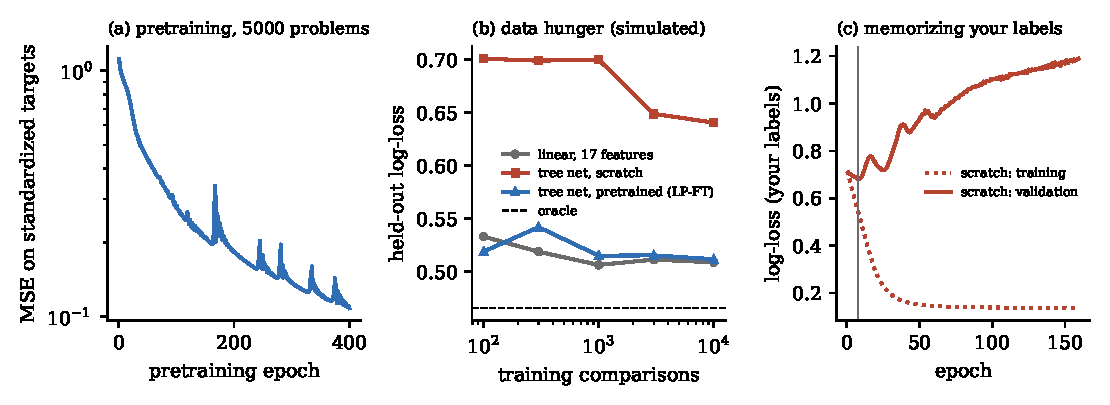
\includegraphics[width=\linewidth]{step11_treenet.pdf}
\caption{(a) Pretraining loss on generated problems. (b) Held-out log-loss vs.\ training comparisons on the simulated instructor. (c) One fold of your labels: the scratch
network's training and validation loss; the vertical line marks early stopping.}\label{fig:step11}
\end{figure}

\paragraph{What to make of a tie.}
Be honest about what the pretrained network knows. Its pretraining targets \emph{were} the hand-made features, so it learned what the feature designer
already knew and then matched the feature model. The gains from learned representations show up when (i) the useful structure is something nobody thought to
make a feature (Exercise~\ref{ex:pretrain}), or (ii) there is far more labeled data than $NNJudg$ judgments. The real lessons of this section are about the
machinery: reverse-mode differentiation through a recursive structure, how quickly a few thousand parameters memorize a few hundred labels, and how to use
cheap data you have in abundance (generated problems) to make expensive data you have little of (your judgments) go further.

\paragraph{Exercises.}
\begin{exercise}
Write out reverse mode for a two-level tree $h_{\text{root}}=\tanh(W_{\sin}h_1+b)$, $h_1=\tanh(W_{\text{pow}}[h_x;n;\dots]+b')$, with loss $L=\ell(v\cdot h_{\text{root}})$. Show that
computing $\nabla_\Theta L$ costs a constant multiple of evaluating $L$, while forward mode would need one pass per parameter.
\end{exercise}
\begin{exercise}\label{ex:sum}
Show that a mean aggregator $\frac1m\sum_kh(u_k)$ gives $u+u$ and $u$ (as summands) the same input, while a sum does not. Which features of Section 3
could a mean-aggregating network not represent?
\end{exercise}
\begin{exercise}\label{ex:pretrain}
Pretraining targets are free to choose. Propose a target that the differentiator can compute but that is \emph{not} among the 17 features (for example, the number of terms in the
\emph{simplified} derivative, or whether simplification cancels anything). Argue why a network pretrained on it might beat the feature model on your labels, and how you would test it.
\end{exercise}

%=============================================================================
\section{Explaining a prediction: Shapley values}
\label{sec:shapley}
%=============================================================================

The model says $A$ is harder than $B$ with probability 0.94. \emph{Why?} Section 9's split gain answered a global version of that question badly. It credits
whichever of several correlated features a tree happened to split on. This section answers the local question, for one comparison, with the only
attribution rule that satisfies four natural axioms. The answer also becomes the explanation the guessing game of Section 13 shows players.

\paragraph{A comparison as a cooperative game.}
Let $f$ map a feature vector to a predicted difficulty, and fix two problems with features $a,b$. Partition the $\FNFeatures$ features into $k=\XNGroups$ groups that
mean one thing to an instructor (size, chain rule, quotient rule, product rule, function types, tricky exponents, powers and constants). These groups are the \emph{players}. A coalition $S$ of
groups ``switches on'' $A$'s values for its groups and leaves the rest at $B$'s:
\[
  v(S)=f(a_S,b_{\bar S})-f(b),\qquad v(\varnothing)=0,\qquad v(\text{all})=f(a)-f(b).
\]
So $v$ interpolates between the two problems, and the question is how to divide the total gap $f(a)-f(b)$ among the groups.

\begin{theorem}[Shapley 1953]
There is exactly one map $v\mapsto\phi(v)\in\R^k$ satisfying
(i) \emph{efficiency}: $\sum_j\phi_j=v(\text{all})$;
(ii) \emph{symmetry}: if $v(S\cup j)=v(S\cup j')$ for all $S\not\ni j,j'$, then $\phi_j=\phi_{j'}$;
(iii) \emph{null player}: if $v(S\cup j)=v(S)$ for all $S$, then $\phi_j=0$;
(iv) \emph{additivity}: $\phi(v+w)=\phi(v)+\phi(w)$. It is
\[
  \phi_j=\sum_{S\not\ni j}\frac{|S|!\,(k-|S|-1)!}{k!}\bigl[v(S\cup j)-v(S)\bigr],
\]
the marginal contribution of $j$ averaged over all $k!$ orders in which the players could arrive.
\end{theorem}
\begin{proof}[Proof sketch]
Games on $k$ players form a vector space of dimension $2^k-1$. The \emph{unanimity games} $u_T(S)=\mathbf 1[T\subseteq S]$, $T\ne\varnothing$, are a basis: Möbius inversion
writes any $v=\sum_Ta_Tu_T$ with $a_T=\sum_{S\subseteq T}(-1)^{|T|-|S|}v(S)$ (the \emph{Harsanyi dividends}). On $c\,u_T$, players outside $T$ are null, so get 0 by (iii), and those inside are
symmetric, so by (i) and (ii) each gets $c/|T|$. This holds for every real $c$, so additivity determines $\phi(v)=\sum_T\phi(a_Tu_T)$ uniquely.
Checking that the permutation formula satisfies (i)--(iv) is direct.
\end{proof}

Efficiency is what makes Shapley values right for \emph{pairs}. With $B$ as the baseline, the attributions add up exactly to the model's predicted gap, so they literally decompose
the log-odds $\hat\delta(A)-\hat\delta(B)=\log\frac{P(A\succ B)}{P(B\succ A)}$. For a \emph{linear} model the game is additive, and the formula collapses to
$\phi_j=\sum_{i\in G_j}\theta_i(a_i-b_i)$ (Exercise~\ref{ex:linshap}). For the boosted model of Section 9 nothing collapses, and we compute the formula exactly.

\paragraph{Exact computation in one vectorized call.}
With $k=\XNGroups$ there are $2^k=\XNCoalitions$ coalitions. Build all $\XNCoalitions$ hybrid feature vectors at once, score them in a single call, and read off every marginal contribution:

\codefrom{src/calcdiff/explain.py}
\begin{lstlisting}
masks = _masks(k)                                  # (2^k, k): row r = binary digits of r
X = np.repeat(b[None, :], len(masks), axis=0)      # start every coalition at B's features
for j, cols in enumerate(groups):
    X[np.ix_(masks[:, j], cols)] = a[cols]         # members of the coalition take A's values
v = f(X) - f(X)[0]                                 # row 0 is the empty coalition
index = masks @ (1 << np.arange(k))                # each coalition's row number
for j in range(k):
    without = ~masks[:, j]                         # all S not containing j
    with_j = index[without] | (1 << j)             # S + j, by setting bit j
    phi[j] = np.sum(weight[size[without]] * (v[with_j] - v[without]))
\end{lstlisting}
Representing coalitions as the bits of an integer makes ``$S\cup\{j\}$'' a bitwise OR, so the whole sum is array indexing. Over 400 random pairs, $\sum_j\phi_j$ matched the model's gap
to within $\XEffErr$, which is efficiency up to floating-point rounding. Tests check every axiom: efficiency on a boosted model, null player (a group the model ignores gets exactly 0),
symmetry (a pure interaction $x_qx_p$ is split $\frac12,\frac12$), and the linear closed form.

When $2^k$ evaluations are too many, average marginal contributions over $n$ random orders instead (\code{shapley\_sampling}). The estimate is unbiased, and each
single order already satisfies efficiency exactly. Its error falls like $n^{-1/2}$. Figure~\ref{fig:step12}(c) measures a slope of $\XSampSlope$, and 20 orders already give an RMS error of $\XSampErrTwenty$ logits.

\paragraph{Why groups?}
Section 6 showed that ridge spreads weight across near-duplicate features (\code{n\_chain} vs.\ the function counts). Per-feature attributions inherit that
arbitrariness. Making the whole family one player sidesteps the question of how to split credit inside it, a question the data cannot answer.
It also makes the explanation say something an instructor recognizes. And it cuts the cost from $2^{17}$ to $2^7$ evaluations.

\paragraph{What drives your model's judgments.}
Figure~\ref{fig:step12}(a) averages $|\phi_j|$ over 400 random pairs of pool problems for the two models fitted to your $\XNJudg$ judgments. For linear BT the largest is the
\emph{\XTopLin} group ($\XTopShareLin\%$ of the total), then \emph{\XSecondLin}. For boosted BT it is \emph{\XTopBst} ($\XTopShareBst\%$), then \emph{\XSecondBst}.
The rankings broadly agree (Spearman $\XRhoLinBst$), but the two models, which predict almost equally well (Sections 8 and 9), divide the credit quite differently.
Breiman called this the \emph{Rashomon effect}: many models fit the data equally well and tell different stories. So Shapley values explain \emph{the model}, not your mind.
When near-duplicate features exist (chain-rule counts and size move together), the data cannot tell which story is true. Split gain is more lopsided still. It gives
\emph{\XGainTopGroup} $\XGainTopShare\%$ of all gain and ranks the quotient group $\XQuotRankGain$th of 7, because it rewards features that are split on often, not features that move predictions.

\paragraph{Explaining single comparisons.}
\code{describe} turns $\phi$ into the sentence a game player will see. It is written from the side of the problem the model judges harder: if $\sum_j\phi_j<0$, it negates $\phi$ first.
My first version forgot this, and for a pair where the model preferred $B$ it cheerfully explained what made $A$ harder.

\codefrom{src/calcdiff/explain.py}
\begin{lstlisting}
def describe(phi, names=None, top=2):
    if phi.sum() < 0:                  # the model picked B: justify B
        phi = -phi
    order = np.argsort(-phi)
    up = [names[j] for j in order[:top] if phi[j] > 0.05]
    down = [names[j] for j in order[::-1][:1] if phi[j] < -0.05]
    ...
    s = "Mostly the " + " and the ".join(up)
    return s + (f", despite the {down[0]}" if down else "") + "."
\end{lstlisting}

Table~\ref{tab:shap} explains three of your comparisons with the final linear model: a confident one, a close call, and one where the model disagrees with you.
Panel (b) draws the first as a waterfall. The gap of $\XWFGap$ logits ($P=\XWFProb$) is built mostly from the quotient rule, with the function types pulling back.
That first row also holds a trap. $\frac{\sqrt{4x^3}}{2x^{3/2}}$ \emph{simplifies to $1$} for $x>0$, so a student who simplifies first does almost no work. The model credits the
quotient rule because none of its 17 features can see ``this cancels''. That is exactly the kind of pretraining target Exercise~\ref{ex:pretrain} asks for, and it is a good
illustration of what explanations are for: they make a model's blind spots visible.

\begin{table}[h]\centering\footnotesize
{\renewcommand{\arraystretch}{1.3}\begin{tabular}{llcp{4.3cm}}
\toprule
you said harder & than & $P$ & why, according to the model \\
\midrule
$\displaystyle x^{-1} + x^{1/2} + \frac{\sqrt{4 x^{3}}}{2 x^{3/2}} + 2$ & $\displaystyle x^{4} + x^{2} + \tan\left(x^{4} - 4\right)$ & 0.94 & \parbox[t]{4.2cm}{\raggedright quotient rule $+1.7$, tricky exponents $+0.9$, function types $-0.8$\\ \emph{Mostly the quotient rule and the tricky exponents, despite the function types.}} \\[6pt]
$\displaystyle 5 x + \left(e^{\ln\left(x^{-2} + 5\right) + 8} - 1\right)^{5}$ & $\displaystyle e^{\cos\left(x^{2} + 8\right) x^{2}} + 9 x^{1/2}$ & 0.58 & \parbox[t]{4.2cm}{\raggedright chain rule $+0.7$, powers and constants $-0.4$, size $+0.3$\\ \emph{Mostly the chain rule and the size, despite the powers and constants.}} \\[6pt]
$\displaystyle x^{2} + \left(\left(x^{1/3} + 3\right)^{4} - 3\right)^{2}$ & $\displaystyle x^{3} + 7 \left(-4 x^{1/2}\right) \sin\left(x^{-1} e^{-5 x^{2} + 1}\right)$ & 0.08 & \parbox[t]{4.2cm}{\raggedright size $-1.6$, function types $-0.6$, powers and constants $+0.5$\\ \emph{Mostly the size and the function types, despite the powers and constants.}} \\[6pt]
\bottomrule
\end{tabular}}

\caption{Shapley explanations of three of your judgments by the final linear model: the three largest group contributions (logits, positive = toward the problem you chose) and the
generated sentence, which justifies the model's own pick. $P$ is the model's probability that the problem you chose is harder.}\label{tab:shap}
\end{table}

\begin{figure}[h]\centering
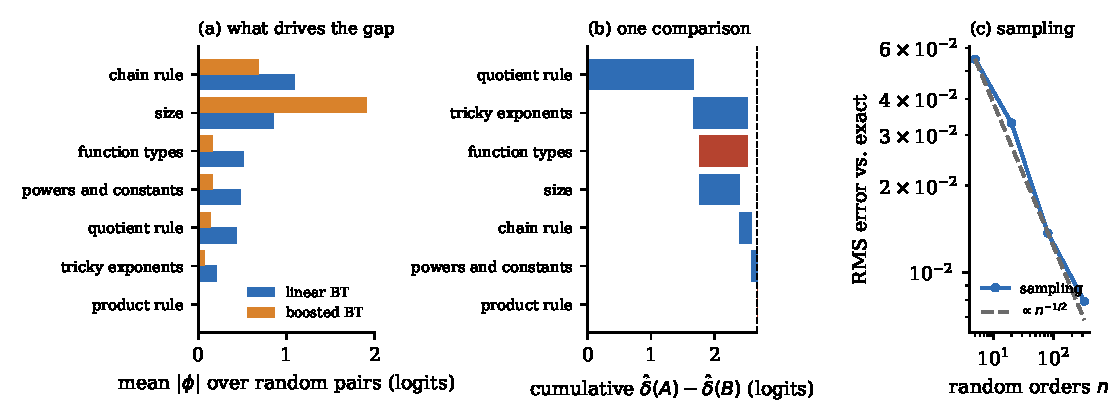
\includegraphics[width=\linewidth]{step12_shapley.pdf}
\caption{(a) Mean $|\phi|$ per feature group over random pairs, for linear and boosted BT fitted to your labels. (b) Waterfall for the first row of Table~\ref{tab:shap}: contributions accumulate
to the predicted gap (dashed). (c) RMS error of the sampling estimator against exact values, vs.\ number of random orders.}\label{fig:step12}
\end{figure}

\paragraph{A caution about hybrids.}
The coalition $v(S)$ evaluates the model on \emph{hybrid} feature vectors: $A$'s chain-rule counts with $B$'s size, say. Some hybrids correspond to no real problem (three nested chain
rules in a five-node tree). The model is then extrapolating, and so is the explanation. Conditional variants of Shapley values avoid this by averaging over realistic
completions, but they need a model of the feature distribution and break the null-player axiom. For explaining a \emph{comparison}, where both endpoints are real problems,
the baseline version used here is the standard choice.

\paragraph{Exercises.}
\begin{exercise}\label{ex:linshap}
Show that for $f(x)=\theta\cdot x+c$ the game is additive, $v(S)=\sum_{j\in S}\sum_{i\in G_j}\theta_i(a_i-b_i)$, and deduce the closed form. Is the converse true: does
$\phi_j(a,b)=\sum_{i\in G_j}\theta_i(a_i-b_i)$ for all $a,b$ force $f$ to be linear?
\end{exercise}
\begin{exercise}
Compute the Harsanyi dividends of $v(S)=f(a_S,b_{\bar S})-f(b)$ for $f(x)=x_1x_2x_3$ with $a=(1,1,1)$, $b=(0,0,0)$, and verify the Shapley values $\frac13$ each. What do the dividends of a boosted
model of depth $D$ look like, and why do they vanish for coalitions larger than $D$?
\end{exercise}
\begin{exercise}
Construct two functions $f,g$ on two binary features with $f=g$ on three of the four corners (``the data'') but different Shapley values for the pair $a=(1,1)$, $b=(0,0)$. Relate this to the
Rashomon effect and to the hybrid caution above.
\end{exercise}

\end{document}
